%!TEX program = xelatex
% =============================================================================
%   paper.tex - PNAS-style draft
%   "The Imagination of Nature: Mythology as the Cultural Recording
%    Layer of Perceptual Coupling"
% =============================================================================
\documentclass[11pt,a4paper]{article}

% Modern Unicode setup (xelatex/lualatex via tectonic).
% Times New Roman has full Cyrillic coverage so the Russian examples
% (медведь, тундра, млекопитающее, etc.) render natively.
\usepackage{fontspec}
\setmainfont{Times New Roman}
\setsansfont{Arial}
\setmonofont{Consolas}
\usepackage[english]{babel}
\usepackage{geometry}
\geometry{margin=1in}
\usepackage{graphicx}
\usepackage{booktabs}
\usepackage{siunitx}
\sisetup{group-minimum-digits=4, output-decimal-marker={.}}
\usepackage{amsmath, amssymb}
\usepackage{microtype}
\usepackage{authblk}
\usepackage{xcolor}
\usepackage[hidelinks,colorlinks=true,citecolor=blue!50!black,linkcolor=blue!50!black]{hyperref}
\usepackage{caption}
\captionsetup{font=small, labelfont=bf, labelsep=period}
\usepackage{natbib}
\bibliographystyle{plainnat}
\usepackage{titlesec}
\titleformat{\section}{\LARGE\bfseries}{\thesection}{1em}{}
\titlespacing*{\section}{0pt}{1.5em plus 0.4em minus 0.2em}{0.8em plus 0.2em}
\titleformat{\subsection}{\Large\bfseries\itshape}{\thesubsection}{0.8em}{}
\titlespacing*{\subsection}{0pt}{1.2em plus 0.3em minus 0.2em}{0.5em plus 0.1em}
\setlength{\parskip}{0pt}
\setlength{\parindent}{1.2em}

\graphicspath{{figures/}}

\title{\bfseries The Imagination of Nature:\\
\large Mythology as the Cultural Recording Layer of Perceptual Coupling}

\author[1]{Antoine Bellemare-Pepin}
\author[2]{Mar Estarellas}
\affil[1]{Department of Psychology, Université de Montréal}
\affil[2]{Department of Psychiatry, McGill University}
\date{\today}

\begin{document}

\maketitle

\begin{abstract}\noindent
Mythography has long treated the symbolic content of myth as a
function of mind and culture, with the biome supplying raw
material but not form. A counter-tradition from Schelling through
Bateson and the ecological anthropology of Descola and Ingold
treats imagination instead as a coupling between perceiver and
environment, on which mythologies should carry a recoverable
trace of their biomes. We test this with Berezkin's catalogue of
folk-motifs from 958 traditions, geocoded to the WWF terrestrial
biomes and aligned via sentence-pooled SigLIP-2 to iNaturalist
species photographs and Places365 landscape scenes after an LLM
pipeline strips species, place, ethnonym, and biome-word
vocabulary from the motif text. The alignment survives on both
image corpora, replicates across four vision--language models,
and decays monotonically with motif breadth, strongest in
biome-specific motifs and fading toward zero in universals. The
pattern is consistent with perceptual coupling at the
lexical-thematic level. The residue mythology carries of its
biome is not a catalogue of names but the schemas of attention,
activity, and form that the biome made available to imagination.
On this reading, mythology functions as the cultural recording
layer of an ongoing engagement between perceiver and environment,
a substrate that survives even when species, place, and biome
words are stripped from the text because the perceptual encounter
shaped the very activities and articulations the narrative is
built from. The breadth gradient is the load-bearing signature.
Biome-specific motifs stabilised in encounter with a particular
ecology and carry that encounter forward into their narrative
substance, while universal motifs propagated only by detaching
from any single biome and stabilising on cross-cultural
structures, so the coupling fades in them precisely as the
lineage from Schelling and Bateson through contemporary 4E
cognitive science would predict. Mythology, on the reading the
data support, is one of the long instruments humans have used to
keep the coupling between cognition and environment articulate
across generations. We advance this stabilisation-over-generations
account as the interpretive thesis the cross-sectional alignment
most naturally motivates, not as a diachronic process the present
correlational data establish on their own.
\end{abstract}

\vspace{0.6em}

% =============================================================================
\noindent\textbf{Significance Statement}\\[0.4em]
Mythologies of cultures inhabiting different biomes carry a recoverable
visual signature of those biomes, even after every species name, place
name, and biome word is stripped from the text. The signature is
strongest in biome-specific myths and attenuates progressively as
motifs propagate across more biomes. The pattern is consistent with
the hypothesis that the ecological structure of a biome contributes
to the stabilisation of its mythological motifs, and reopens, in
empirically tractable form, a two-century-old debate over whether
imagination is a private projection of cultural meaning onto a
passive world or a coupling phenomenon between perceiver and
environment.

\vspace{1em}

% =============================================================================
\section*{Introduction}

Modern thought has long treated nature as a passive backdrop onto
which the human mind projects meaning. Mythology, on this view, is
what humans \emph{do to} a world, a projection of cultural
categories, anxieties, and social structures onto matter. The biome
a culture inhabits supplies raw material but not, on this reading,
the \emph{form} of its symbols. We call this dominant view the
\emph{projection account}. Running parallel to this default, however,
a different tradition has insisted on a different picture.
Schelling's distinction between \emph{natura naturata} (nature as
finished product) and \emph{natura naturans} (nature as productive
activity)~\citep{schelling1797ideas,schelling1799outline} was
recovered in the twentieth century by Bateson's claim that ``mind is
wherever the conditions for a mental process obtain'' across coupled
systems, where differences make differences and pattern propagates
between brain, body, environment, and
culture~\citep{bateson1972steps,bateson1979mind}. Depth psychology
made a related move. Jung's mature view of the archetypes resisted
easy translation into innate mental contents stored in individual
brains and instead located them in the joint between psyche and
nature~\citep{jung1959archetypes}; Hillman radicalised this into
archetypal psychology and the recovery of \emph{anima
mundi}~\citep{hillman1975revisioning,hillman1981thought}; Henri
Corbin gave it its most precise philosophical name in the \emph{mundus
imaginalis}, the imaginal world, distinct from the modern collapse
of ``imaginary'' into ``merely
subjective''~\citep{corbin1972mundus,barfield1957saving,abram1996spell,ingold2000perception}.
The thread connecting these authors is that imagination is a
perceptual organ rather than a productive one, an organ that
discloses content present in the encounter between an attentive
perceiver and an articulate world. We call this opposing view the
\emph{coupling account}, since on this reading perceiver and
environment co-produce symbolic content together.

Since the 1960s the cognitive sciences have been producing the
empirical scaffolding for exactly this coupling view. Gibson's
ecological psychology replaced the dominant representational model
of perception with one of \emph{direct pickup}, in which the
environment is information-rich at the level of the optic array and
the organism tunes itself to a richly structured world that already
contains the relevant
information~\citep{gibson1979ecological}. The 4E framework
(embodied, embedded, extended, and enactive cognition) generalised
this beyond
perception~\citep{varela1991embodied,clark1998extended,noe2004action}.
Predictive processing supplied the neural substrate, with the brain
treated as a hierarchical prediction machine that locks onto
interpretations its priors privilege, given the actual statistical
structure of what the world
presents~\citep{friston2010free,clark2016surfing,hohwy2013predictive}.
On this account pareidolia is not a mistake of perception but the
system working as designed. Niche construction theory closed the
loop~\citep{odlingsmee2003niche}, observing that humans produce
symbolic environments (names, stories, transmitted practices) and
that these environments shape the cognition of subsequent generations.

The two accounts make different empirical predictions about
mythology. The projection account treats the symbolic content of
myth as largely a product of mind and culture, and therefore
predicts that once the text of a mythology has been stripped of its
overt environmental and cultural anchors (species names, place
names, ethnonyms, biome words, climate phrases, tradition labels),
the residual narrative should carry no detectable visual signature
of the biome the tradition inhabits.
On this reading, what remains of mythology after anonymisation is
the cross-cultural grammar of plot and relation, and that grammar
should be indifferent to which biome a tradition emerged in. The
coupling account treats imagination instead as a perceptual organ
jointly tuned by mind and environment, and therefore predicts that
the structural character of a biome, its light, its dominant forms,
its taxa, the affordances it presents to a perceiver, should leave
a recoverable residue in the surviving text, because that residue
was part of what stabilised the mythology in the first place. A
secondary prediction that follows more naturally from the coupling
reading than from the projection reading is that this residue
should be strongest in motifs whose distribution remained close to
a single biome and attenuate as motifs propagate across many
biomes, since universally-shared motifs are precisely those whose
stabilising encounters were not tied to one environment.

Two recent developments make this question newly testable at scale.
The first is the cross-cultural folk-motif catalogue assembled by
Yu.\ E.\ Berezkin, comprising 2{,}564 motifs across 958 traditions
with Russian-language abstracts and geocoded
centroids~\citep{berezkin2024catalogue}, which we have joined to the
WWF Ecoregions classification of 14 terrestrial
biomes~\citep{olson2001terrestrial}. The second is the development of
frontier vision--language models such as
SigLIP-2~\citep{tschannen2024siglip2}, which embed text and image in a
shared metric space learned from billions of image--text pairs sampled
from the internet. The combination lets us ask whether, after
stripping every species name, every place name, every biome word, and
every tradition label, the embedding of a tradition's mythology
preferentially aligns with images of its own biome, and whether
that alignment is concentrated in biome-specific motifs in the
way an ecological-affordance reading would predict.

We report below that such a residue is detectable. After stripping
every overt environmental and cultural anchor from the text, the embedding of a tradition's mythology
preferentially aligns with images of its own biome on two
independent image corpora and across four vision--language model
architectures, in both Russian and English. The alignment is
graded with motif breadth in the way an ecological-affordance
reading would predict, strongest in motifs that did not propagate
beyond a single biome and attenuating in motifs shared across
many. We take this pattern to be more naturally accommodated by a
coupling or ecological-affordance account than by a view in which
biome supplies only interchangeable narrative material, and read
mythology as the surviving textual residue of an ongoing
perceptual coupling between cognition and environment, the
recoverable trace in transmitted narrative of a living engagement
that the narrative itself does not exhaust.

% =============================================================================
\section*{Results}

\begin{figure}[h!t]
\centering
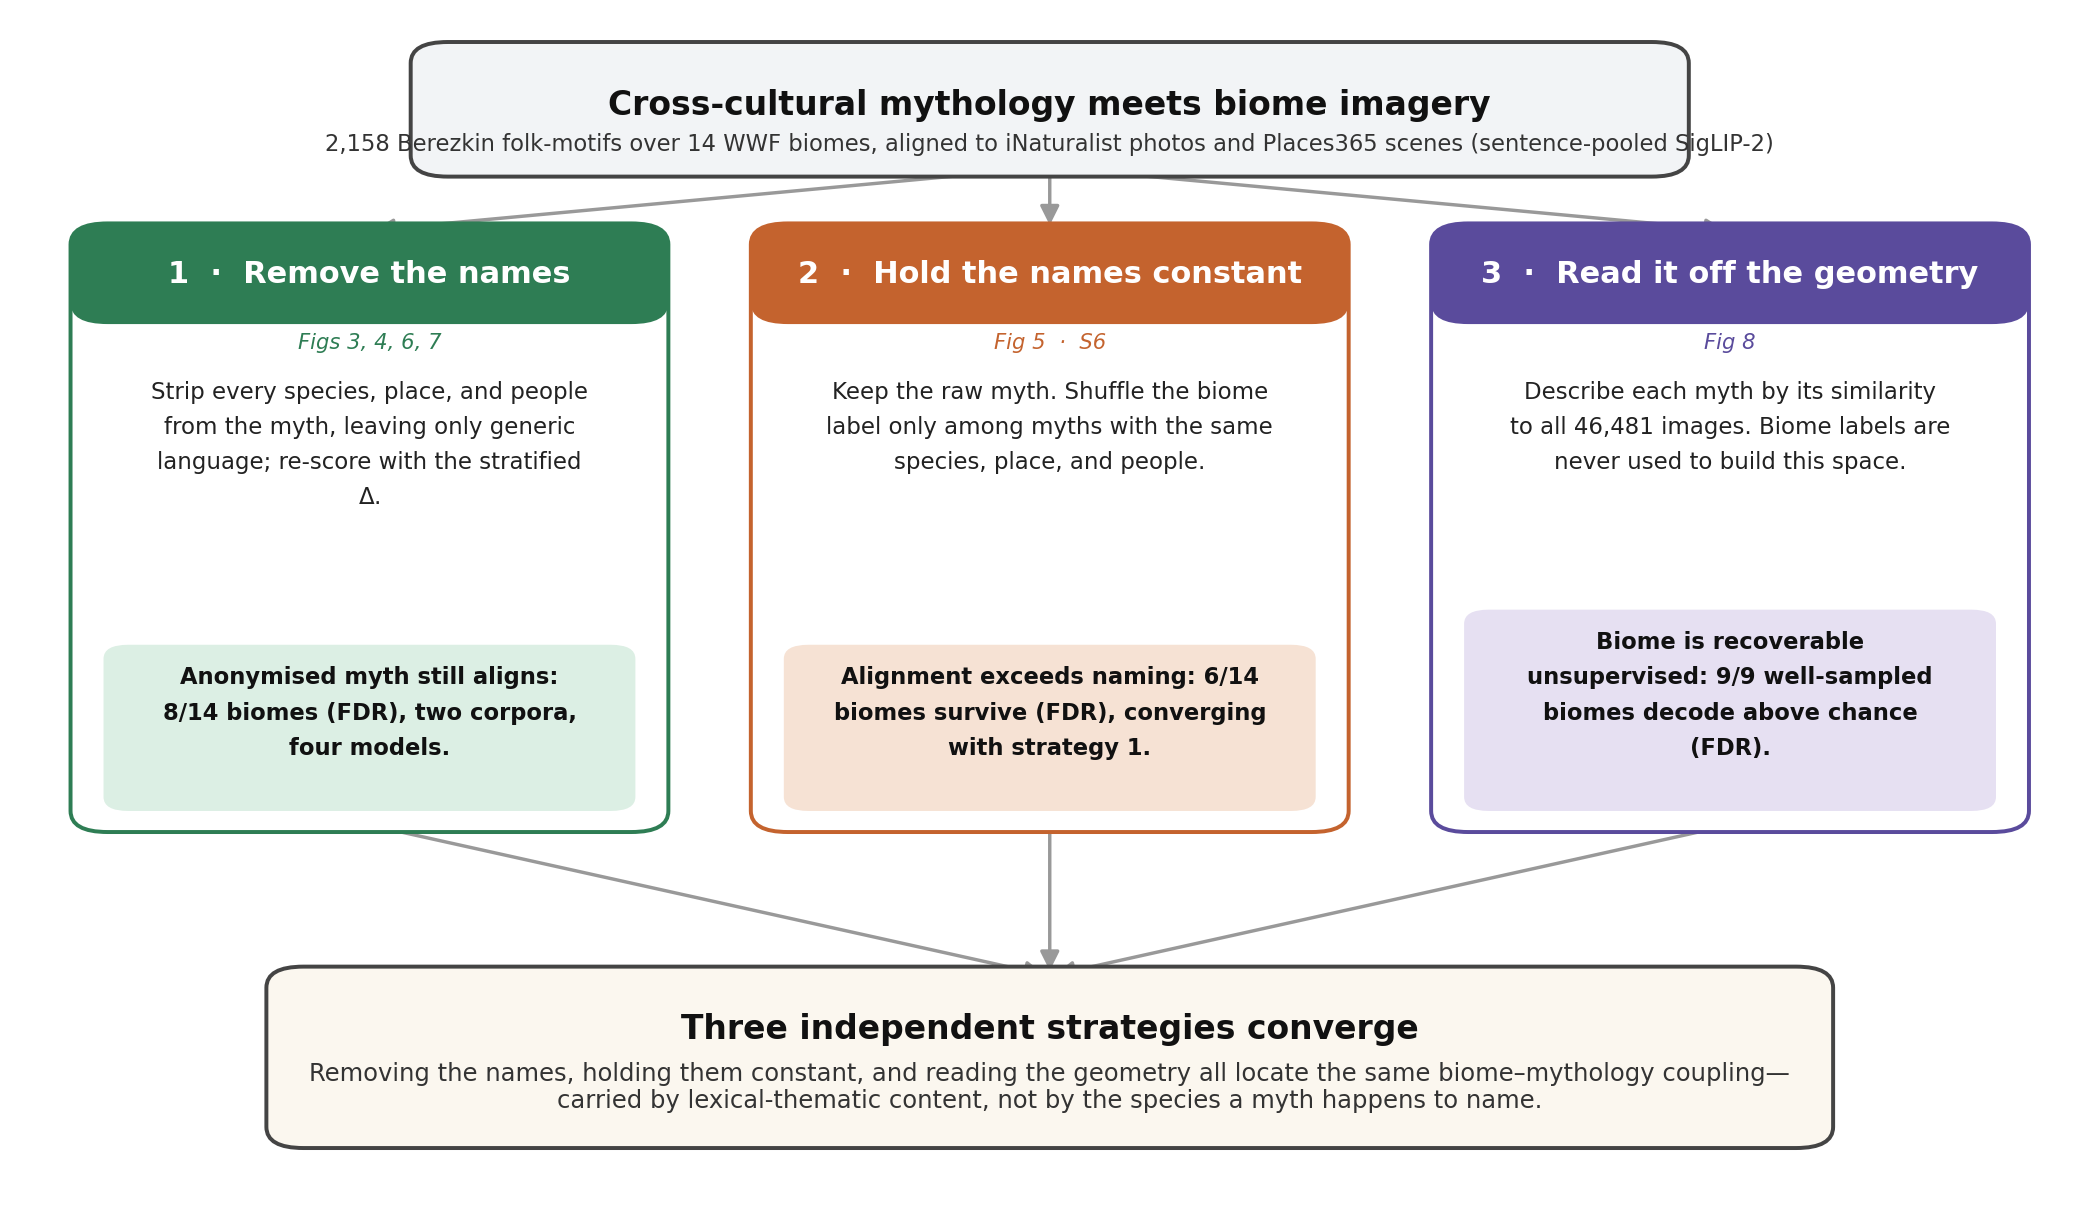
\includegraphics[width=\textwidth]{fig_roadmap.png}
\caption{\textbf{Three independent strategies for asking whether
mythology carries a trace of its biome.} We test the same
question three ways whose assumptions do not overlap.
\emph{(1)~Remove the names}: anonymise the text (every species
$\rightarrow$ its class word, place and ethnonym $\rightarrow$ a
placeholder, biome words dropped) and measure the
within-iconic-taxon stratified alignment to biome imagery.
\emph{(2)~Hold the names constant}: keep the raw myths intact and
break the biome--identity correlation with a matched-permutation
null that shuffles biome only among motifs of like species, place,
and ethnonym content. \emph{(3)~Read it off the geometry}:
describe each myth by its similarity profile across the whole
image set and recover biome structure without ever using biome
labels to build the representation. The three strategies converge
on the same biome--mythology coupling, carried by lexical-thematic
content rather than by the species a myth happens to name. The
figure pointers index the Results subsections that follow.}
\label{fig:fig-roadmap}
\end{figure}

\subsection*{Biome-specific mythology aligns with biome imagery}

\begin{figure}[h!t]
\centering

\includegraphics[width=\textwidth]{fig1_world_traditions.png}
\caption{\textbf{Cross-cultural sample of mythology over the world's
biome geography.} World map of the 958 Berezkin traditions plotted as
dots over the underlying WWF Ecoregions polygons, both coloured by the
same biome palette: continents in semi-transparent biome fills (the
Saharan and Australian deserts in tan, the Amazonian and Indo-Malay
rainforests in dark green, the Boreal belt across northern Eurasia and
Canada in muted blue, Mediterranean basins in red, etc.), tradition
centroids as opaque dots in the same palette. The overlay shows how
densely each biome's actual extent is sampled by Berezkin's corpus.
Eurasian and North American traditions are relatively dense; some
biomes (Mangroves, Flooded Grasslands and Savannas) are sparsely
covered.}
\label{fig:fig1}
\end{figure}

\begin{figure}[h!t]
\centering
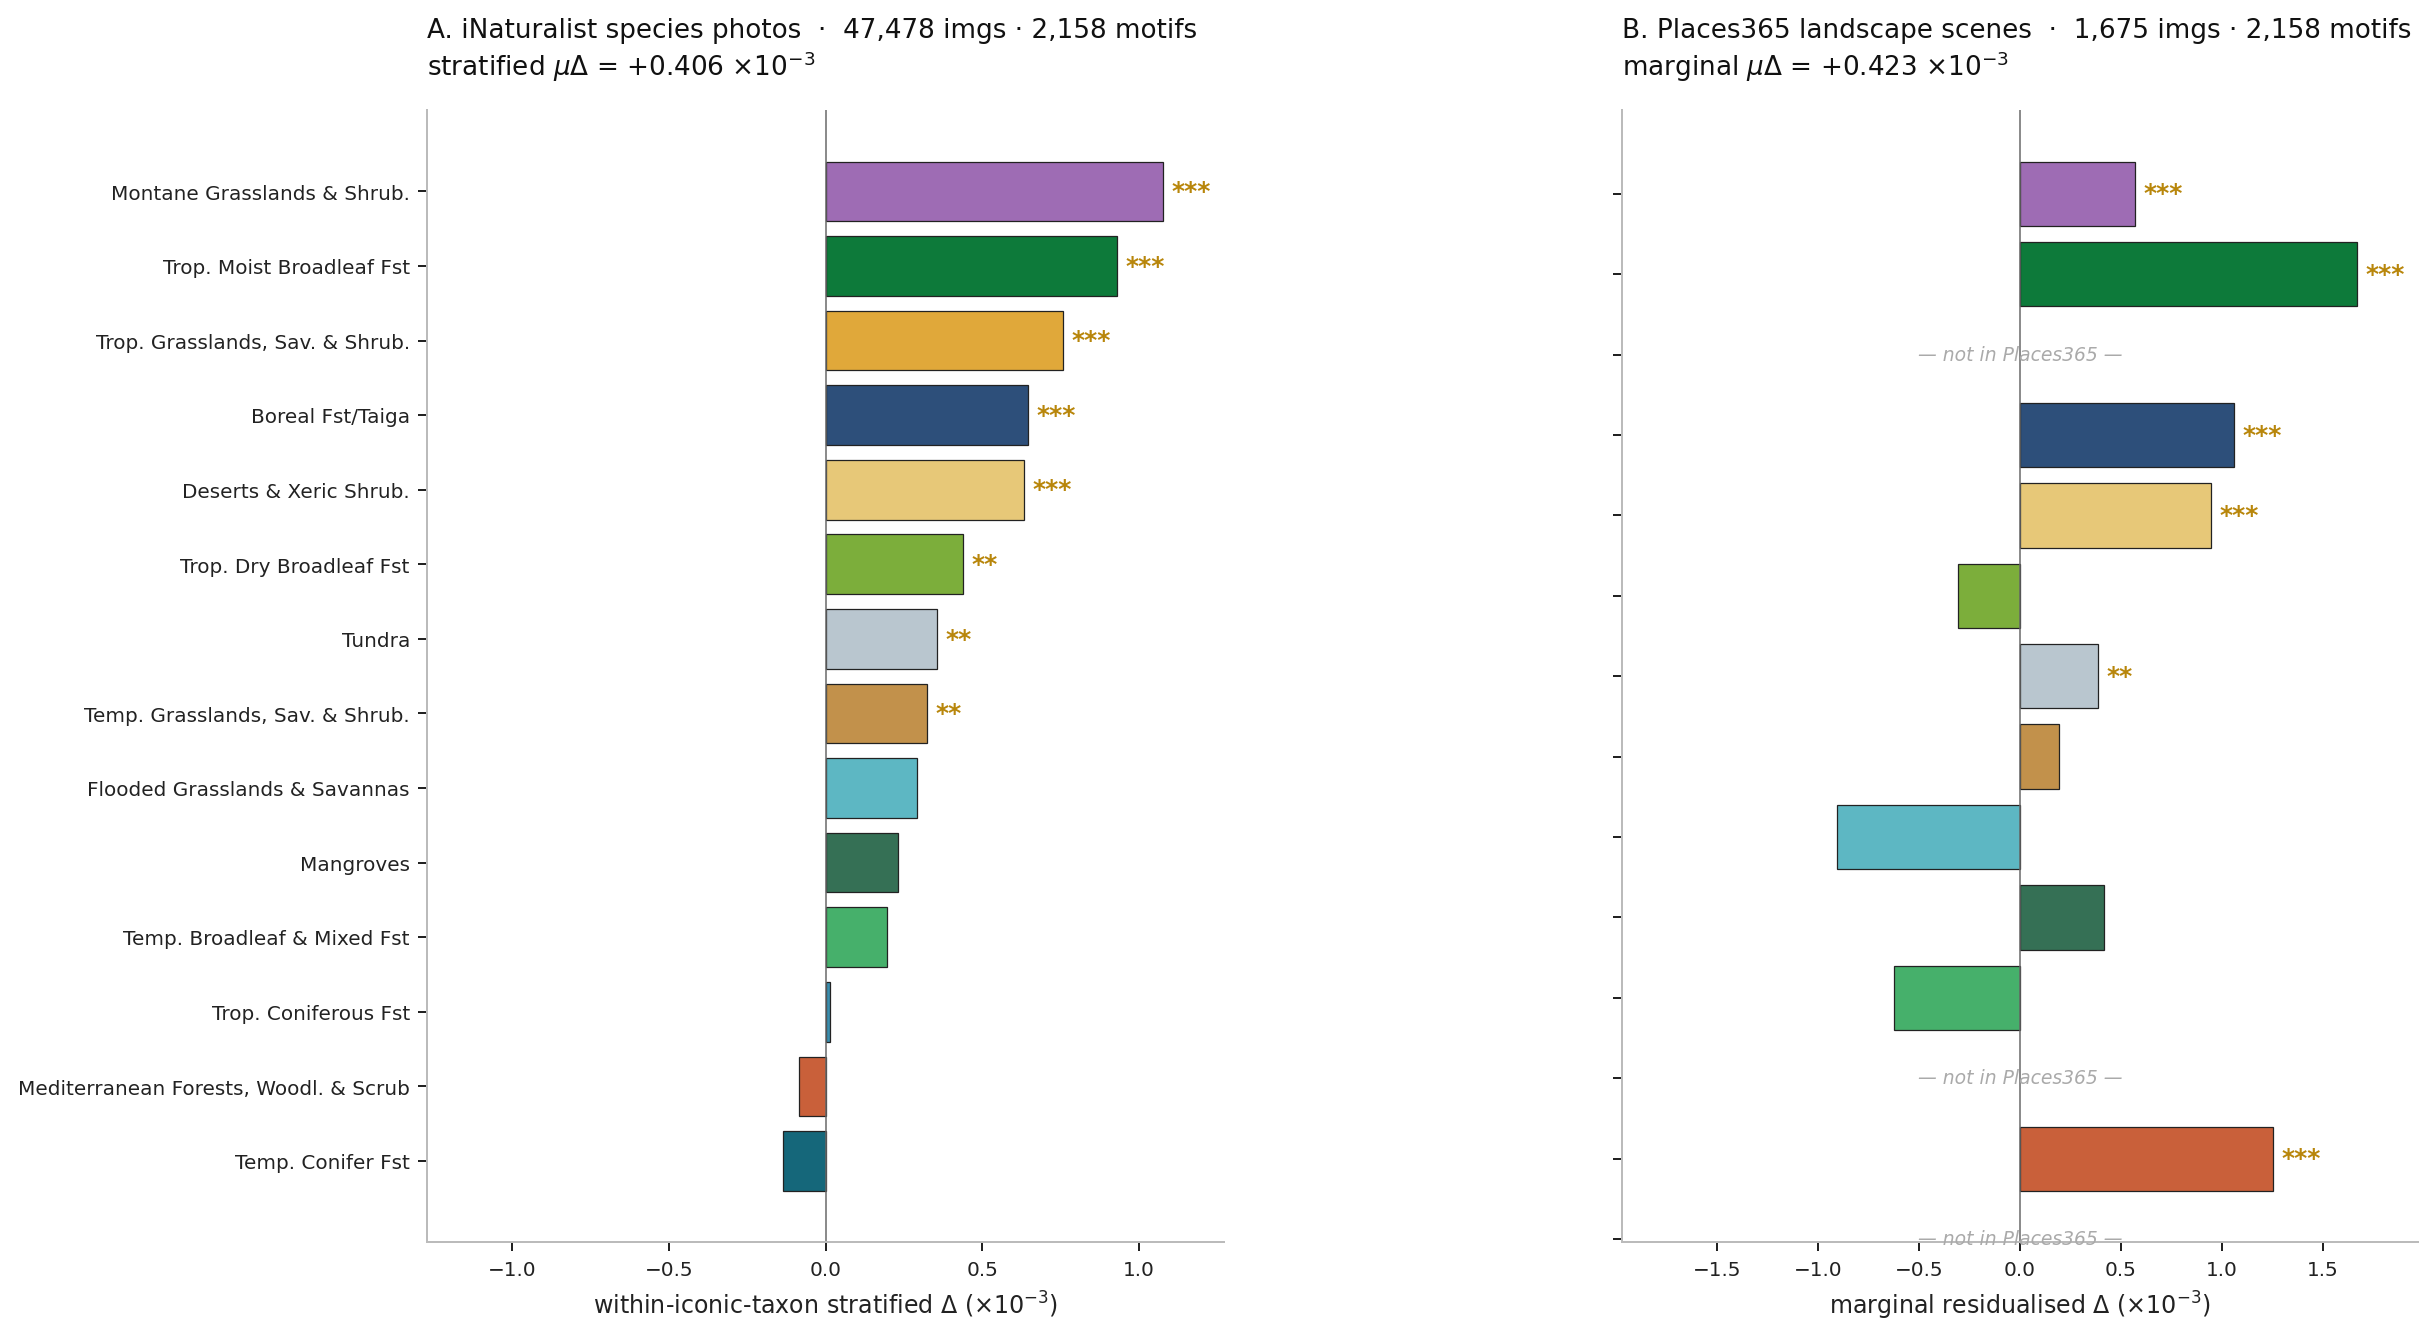
\includegraphics[width=\textwidth]{fig2_biome_bars.png}
\caption{\textbf{The headline coupling signature, replicated on two
independent image corpora.} Residualised $\Delta$ per WWF biome
under sentence-pooled SigLIP-2 on the full LLM-clean Berezkin
abstracts ($2{,}158$ motifs). \emph{Panel A}: iNaturalist species
photographs ($n=46{,}481$ images), with $\Delta$ stratified within
each iconic-taxon stratum and uniformly averaged across taxa to
remove biome--by--iconic-taxon co-occurrence as a possible
explanation; stratified $\mu\Delta = +0.406\times 10^{-3}$, 8/14
biomes significant at $p<.05$. \emph{Panel B}: Places365
strict-landscape scenes ($n=1{,}655$ images, 11 biomes); because
Places365 has no iconic-taxon labels (it is scene-only imagery),
we report the marginal residualised $\Delta$; marginal $\mu\Delta
= +0.423\times 10^{-3}$, 6/11 biomes significant at $p<.05$.
Biomes are ordered top-to-bottom by descending iNat stratified
$\Delta$; biomes Places365 does not cover are blanked. Each panel
uses its own dynamic range. Gold bold asterisks denote
significance after Benjamini--Hochberg FDR correction ($q<.05$);
grey asterisks would denote biomes nominally significant at $p<.05$
but not surviving FDR, of which there are none here (every marked
biome survives FDR, iNat $8/8$ and Places365 $6/6$). The two corpora agree on
the biomes that drive the effect (Tropical Moist Broadleaf,
Deserts, Boreal/Taiga, Montane Grasslands, Tropical Grasslands),
an independent landscape-channel replication of a signal first
recovered on species-channel photographs.}
\label{fig:fig2}
\end{figure}

\begin{figure}[h!t]
\centering
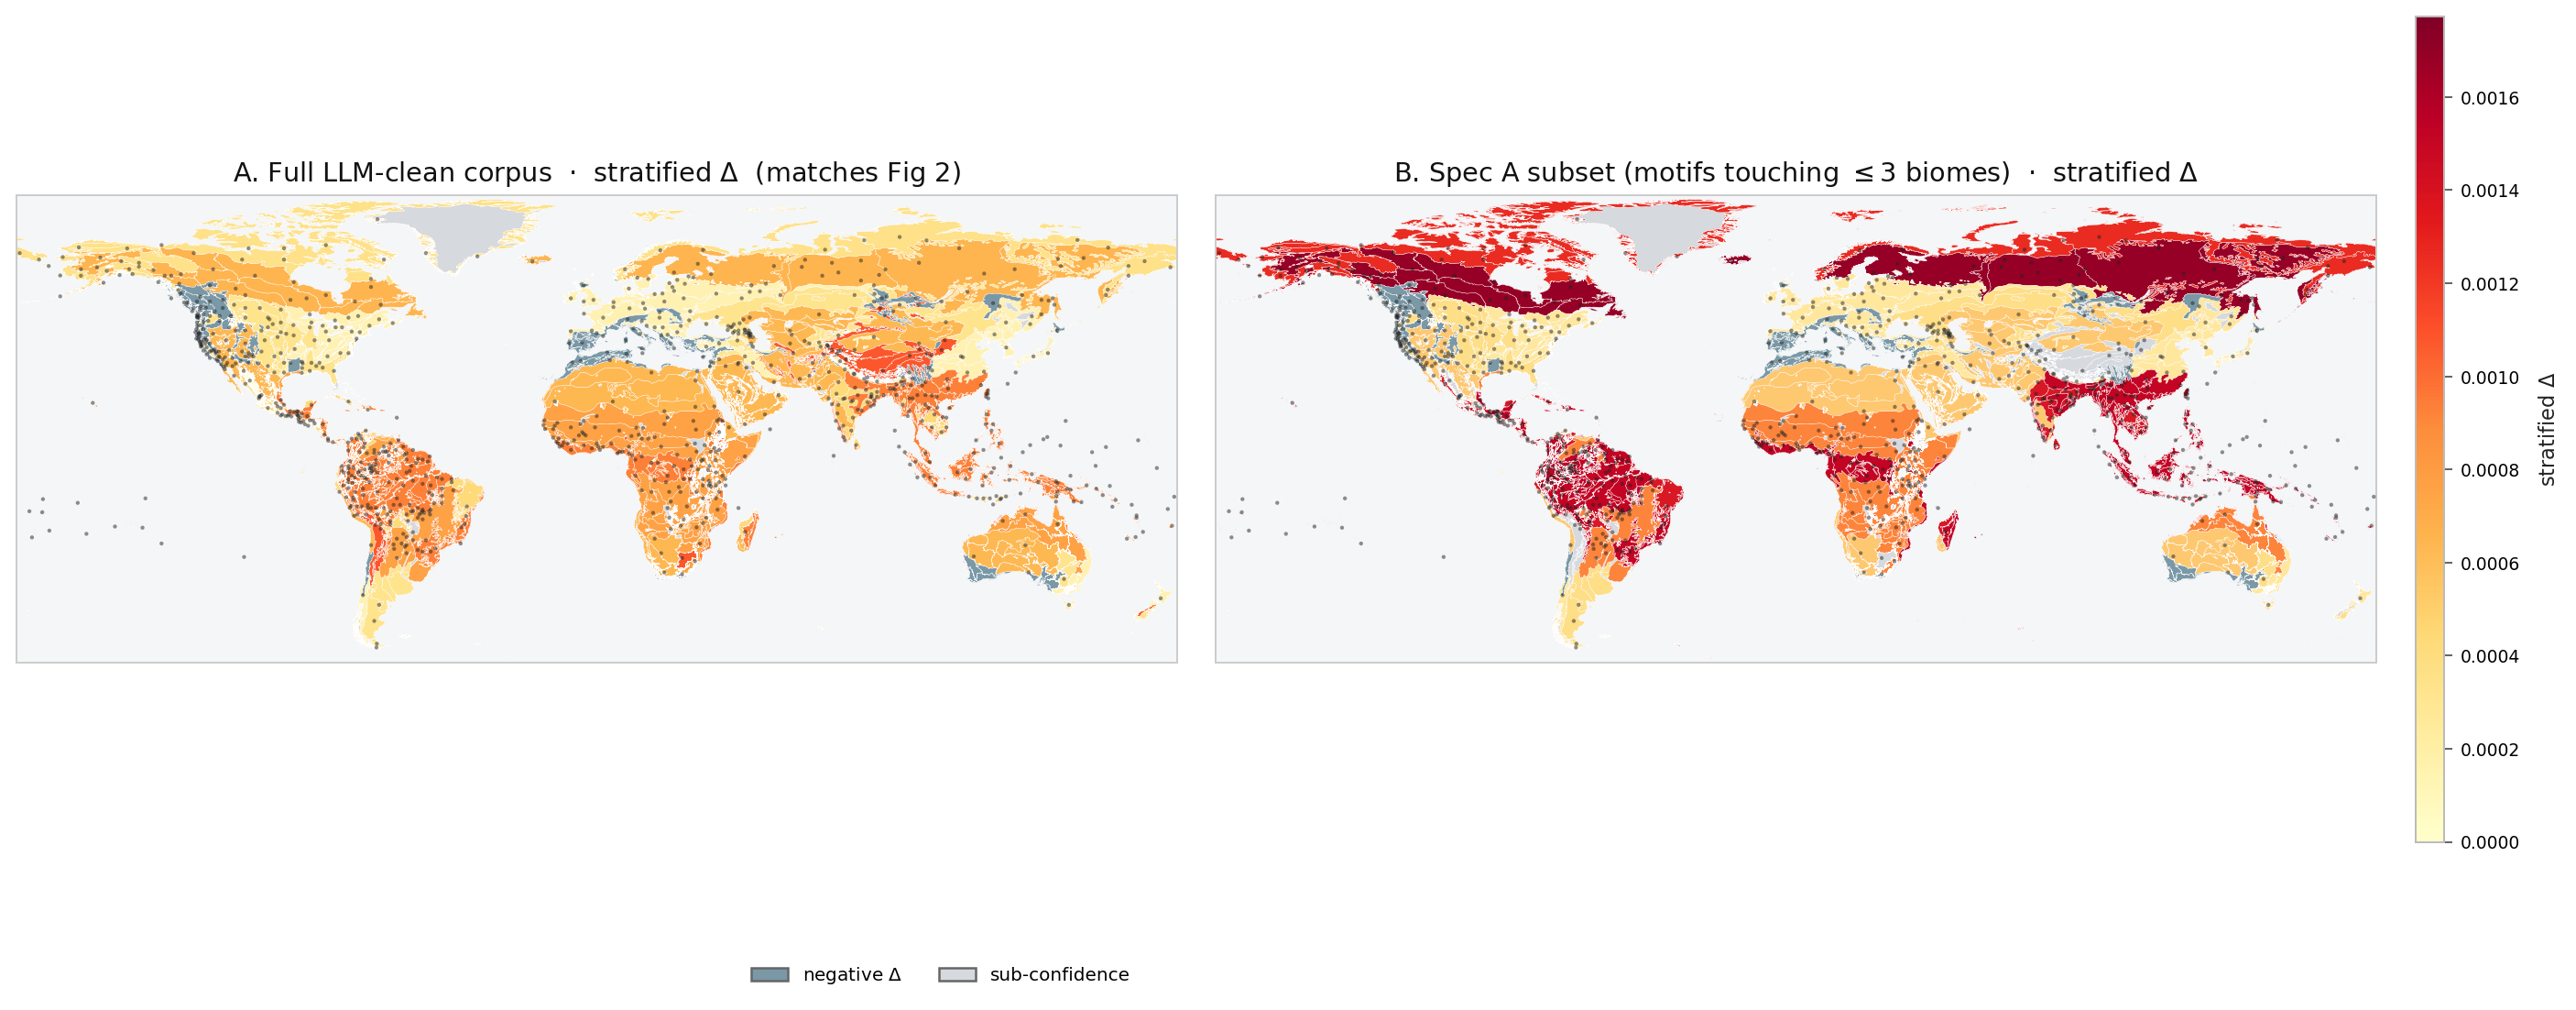
\includegraphics[width=\textwidth]{fig5_earth_map.png}
\caption{\textbf{Per-biome $\Delta$ projected onto the world
map.} Geographic companion to Figure~\ref{fig:fig2}, on the
within-iconic-taxon stratified $\Delta$ under sentence-pooled
SigLIP-2. \emph{Panel A}: full LLM-clean corpus ($2{,}158$
motifs), matching the headline statistic of Figure~\ref{fig:fig2},
Panel A. \emph{Panel B}: Spec A subset (motifs touching $\leq 3$
biomes), the breadth-restricted view that the coupling reading
predicts should show the cleanest geography (cf.\
Figure~\ref{fig:fig11univ}). Colour intensity scales with
stratified $\Delta$ further weighted by confidence ($1 - p$); the
YlOrRd colormap is shared between panels so cell intensities are
directly comparable. Light grey marks sub-confidence biomes
(fewer than $10$ traditions, $50$ motifs, or $50$ photographs);
muted slate-blue marks the rare biomes whose stratified $\Delta$
falls below zero (in panel A, Mediterranean Forests and
Temperate Conifer Forests). Black dots overlay the 958 tradition
centroids. The headline coupling geography appears in both
panels (Tropical Moist Broadleaf rainforests of the Amazon and
Indo-Malay, Tropical Grasslands of sub-Saharan Africa, Boreal
Forests/Taiga of northern Eurasia and Canada, Deserts of North
Africa and central Australia, Montane Grasslands of the
high-altitude tropics) and is substantially more vivid in the
Spec A panel where breadth dilution is removed.}
\label{fig:fig5earth}
\end{figure}

The Berezkin corpus distributes 958 traditions across the 14 WWF
biomes (Figure~\ref{fig:fig1}). After the full anonymisation
pipeline described in \emph{Materials and Methods}, the
LLM-mediated translation and double-pass refinement that replaces
every species with a class word, every place and ethnonym with a
placeholder, and every tradition-specific character name and
cultural-religious title with a neutral generic, the residualised
alignment on the full LLM-clean corpus ($2{,}158$ motifs,
sentence-pooled SigLIP-2) reaches within-iconic-taxon stratified
$\mu\Delta = +0.406\times 10^{-3}$ across the 14 biomes on
iNaturalist (Figure~\ref{fig:fig2}, Panel A; 8/14 biomes
significant at $p<0.05$). The strongest positive cells under
stratification lie in Montane Grasslands \& Shrublands
($\Delta^{\text{strat}} = +1.08\times 10^{-3}$, $p<.001$),
Tropical \& Subtropical Moist Broadleaf Forests
($+0.93\times 10^{-3}$, $p<.001$), Tropical \& Subtropical
Grasslands, Savannas \& Shrublands ($+0.76\times 10^{-3}$,
$p<.001$), Boreal Forests/Taiga ($+0.65\times 10^{-3}$, $p<.001$),
Deserts \& Xeric Shrublands ($+0.63\times 10^{-3}$, $p<.001$),
Tropical \& Subtropical Dry Broadleaf Forests ($+0.44\times
10^{-3}$, $p<.01$), Tundra ($+0.36\times 10^{-3}$, $p<.01$), and
Temperate Grasslands, Savannas \& Shrublands ($+0.33\times
10^{-3}$, $p<.01$). The remaining biomes are positive or near
zero with the exception of Mediterranean Forests and Temperate
Conifer Forests, both weakly negative under stratification.

The biomes that survive the within-iconic-taxon control therefore
carry alignment that is not attributable to biome-by-iconic-taxon
co-occurrence on the image side; the cells where stratification
narrows the marginal effect precisely identify where the marginal
signal was riding on taxonomic composition rather than on
biome-character imagery. Mediterranean Forests is the cleanest
example: its marginal $\Delta = +0.51\times 10^{-3}$ ($p<.001$) is
carried by a single strongly positive Plantae cell ($+1.38\times
10^{-3}$ under the per-taxon decomposition, Figure~\ref{fig:fig10}),
because Mediterranean iNaturalist imagery is dominated by plants
(vineyards, olive groves, shrubland) and the motifs assigned to
Mediterranean biomes lean similarly plant-coded. Once we hold
iconic-taxon fixed on the image side, the Plantae contribution is
uniformly averaged against the negative Aves ($-0.81$), Animalia
($-1.12$), Reptilia ($-0.39$), and Amphibia ($-0.91$) cells, and
the stratified $\Delta$ collapses to $-0.09\times 10^{-3}$ (panel
A bottom). The reverse case is also visible. Boreal Forests/Taiga
has a near-zero marginal $\Delta$ ($+0.03\times 10^{-3}$) because
its dominant Plantae stratum (conifer imagery) carries no
distinctive boreal mythological content; once stratification
gives Mammalia (bears, wolves, $+1.77\times 10^{-3}$) and
Actinopterygii ($+1.39$) equal weight, the boreal $\Delta$
emerges at $+0.65\times 10^{-3}$ ($p<.001$).

The same pattern replicates on an independent image corpus. The
Places365 strict-landscape comparison set, $1{,}655$ scene
photographs across 11 biomes drawn from Places365 scene categories
that unambiguously match a single WWF biome and then
SigLIP-filtered against humans, vehicles, buildings, and close-up
animal subjects, gives a marginal $\mu\Delta = +0.423\times 10^{-3}$
across 11 biomes, with 6 biomes significant at $p<0.05$
(Figure~\ref{fig:fig2}, Panel B). The strongest cells fall in
Tropical \& Subtropical Moist Broadleaf Forests ($\Delta = +1.67
\times 10^{-3}$, $p<.001$), Mediterranean Forests, Woodlands \&
Scrub ($+1.25\times 10^{-3}$, $p<.001$), Boreal Forests/Taiga
($+1.06\times 10^{-3}$, $p<.001$), Deserts \& Xeric Shrublands
($+0.94\times 10^{-3}$, $p<.001$), and Montane Grasslands \&
Shrublands ($+0.57\times 10^{-3}$, $p<.001$). Crucially, the two
corpora cover different visual content: iNaturalist samples close
to species-level (foliage, fauna, fungi in their habitat),
Places365 samples wide-shot terrain with no species or human
subjects. The fact that anonymised mythology aligns above
permutation chance with both channels of biome imagery,
species-level and scene-level, means the alignment is not an
artefact of one corpus's curatorial peculiarities. The per-biome
pattern is likewise not an artefact of a single encoder: it
correlates across four vision--language models (SigLIP-2, M-CLIP,
and OpenCLIP under LAION-2B and OpenAI pretrainings), with
across-model rank correlations of the per-biome $\Delta$ in the
range $r=0.74$--$0.94$, though the two OpenCLIP variants carry a
weaker overall mean (Supplementary Section~S3,
Figure~\ref{fig:figS-crossmodel}). Projected onto
a world map (Figure~\ref{fig:fig5earth}), the warmest cells
concentrate in the Amazonian and Indo-Malay Tropical Moist
Broadleaf rainforests, the Saharan and Australian deserts, the
Mediterranean basins of southern Europe and the western Maghreb,
the boreal belt across northern Eurasia and Canada, and the
montane grassland systems of the high-altitude tropics.

\subsection*{Cultural-geographic autocorrelation}

Mythologies, traditions, and biomes are spatially and
historically clustered. A biome effect could in principle
reflect macroarea, language family, colonial documentation
history, or cultural phylogeny rather than ecological coupling.
To probe this we ran a within-Glottolog-macroarea biome-swap
null. Each Berezkin tradition was assigned to one of six
Glottolog macro-areas (Africa, Australia, Eurasia, North
America, Papunesia, South America) based on its centroid
coordinates. For each of $1{,}000$ permutations, every
tradition's motifs were randomly reassigned to a \emph{different}
biome from among those represented in its own macro-area: the
tradition's macro-area was preserved and its biome label
shuffled, so within-macroarea cultural autocorrelation and the
colonial documentation history that tracks it remained intact
while biome assignment broke. We then recomputed the within-
iconic-taxon stratified $\Delta$ under each swap. The cross-
biome mean attenuates by roughly half but does not vanish, and
six of the 14 biomes retain observed stratified $\Delta$ above
the $95$th percentile of the swap-null distribution at $p<.05$:
Montane Grasslands \& Shrublands (observed $+1.08\times 10^{-3}$,
swap-null mean $+0.09$, $p<.001$), Tropical \& Subtropical Moist
Broadleaf Forests ($+0.93$ vs $-0.16$, $p<.001$), Boreal
Forests/Taiga ($+0.65$ vs $+0.08$, $p<.001$), Deserts \& Xeric
Shrublands ($+0.63$ vs $+0.22$, $p=.018$), Tropical \&
Subtropical Grasslands \& Savannas ($+0.76$ vs $+0.45$,
$p=.019$), and Temperate Grasslands, Savannas \& Shrublands
($+0.33$ vs $+0.02$, $p=.022$). The full per-biome table and
the visualised swap-null distributions are reported in
Supplementary Section~\ref{sec:biome-tell} and
Figure~\ref{fig:figS-biome-tell}. We do not separately preserve
language family in this null because many language families in
Berezkin's catalogue touch only one or two biomes and admit no
swap target; macro-area is the level at which the test has
statistical purchase across all 14 biomes. Geographic and
cultural autocorrelation therefore contribute to the headline
effect but do not exhaust it: the biome content of the motif
text carries information beyond within-macroarea cultural-region
membership.

\subsection*{The alignment is not reducible to identity naming}

The most direct objection to the headline is that a biome's
mythology simply names that biome's species, places, and peoples,
and the encoder reads the alignment off those names. The
anonymisation pipeline answers this by \emph{removing} the names.
A complementary strategy keeps the original myths intact and
instead \emph{holds the names constant} statistically, on the same
within-iconic-taxon stratified $\Delta$ as the headline so the two
are directly comparable. We extract three identity classes per
motif from the raw Russian text and keep them separate: the species
named in the myth (LLM extraction, adversarial audit $96.7\%$
recall and $95.3\%$ precision), the WWF-codable geographic regions
from Berezkin's metadata, and the ethnolinguistic groups that carry
the motif. Each is embedded as a bag of its entities with the same
sentence-pooled SigLIP-2 pipeline and scored against the same
iNaturalist images (Figure~\ref{fig:fig-identity}).

Each identity channel is biome-diagnostic on its own
(Figure~\ref{fig:fig-identity}A). A species-only bag gives
stratified $\mu\Delta = +0.97\times 10^{-3}$ ($13/14$ biomes
significant), an ethnonym-only bag $+0.73\times 10^{-3}$ ($14/14$),
and a place-only bag $+0.36\times 10^{-3}$ ($14/14$). The full
original myth gives $+0.42\times 10^{-3}$ ($10/14$), close to the
$+0.41\times 10^{-3}$ the \emph{anonymised} corpus reaches on the
same statistic --- two opposite roads, removing the names and
keeping them, of comparable magnitude (the raw-Russian and
English LLM-clean frames are not formally comparable, so we read
the closeness as suggestive rather than identical; see
\emph{Materials and Methods}). A bag of
species names is in fact more biome-diagnostic than the full myth,
which dilutes the species cue with narrative content, and this
holds under stratification, so it is not an artefact of image-side
taxon composition. Species naming is therefore a genuinely strong
biome channel, exactly the concern.

We test whether the full-myth alignment exceeds what that naming
determines, in two independent ways. A matched-permutation null
(Figure~\ref{fig:fig-identity}B) shuffles biome labels only among
motifs that are nearest neighbours in the relevant identity-bag
embedding ($60$ K-means blocks), holding identity approximately
constant while breaking biome, and recomputes the stratified
$\Delta$. Six of the fourteen biomes retain alignment above a joint
null that holds species, place, and ethnonym constant
simultaneously --- Tropical Moist and Tropical Dry Broadleaf
Forests, tropical grasslands and savannas, montane grasslands,
boreal forest, and mangroves, with five of these surviving every
single-channel control as well (Figure~\ref{fig:fig-identity}B).
This is the same count as survive the Glottolog cultural-geographic
swap, with four of the six biomes shared between the two lists ---
two stringent and unrelated controls leaving the same handful of
biomes standing. (The place
channel alone is near-circular, since biome is derived from the
region metadata, so we read the joint and species-only nulls rather
than place.) An independent embedding-space test
(Figure~\ref{fig:fig-identity}C) projects the top species-subspace
directions out of the full-myth embeddings and recomputes the
stratified $\Delta$, which attenuates from $+0.42$ to
$+0.20$--$0.27\times 10^{-3}$ but stays significant in $8$ to $12$
of $14$ biomes across $5$, $10$, and $20$ removed directions.
Neither the matched-permutation null nor the linear projection is
an exact control, and both attenuate the effect. What they jointly
establish, from assumptions that do not overlap with the
anonymisation --- the anonymisation route trusts the cleaning but
removes the taxon confound, this route trusts no cleaning and, on
the stratified statistic, removes it too --- is that the
alignment on the un-anonymised myths is not reducible to the
trivial channel by which a biome's mythology names its own
species, places, and peoples.

\begin{figure}[h!t]
\centering
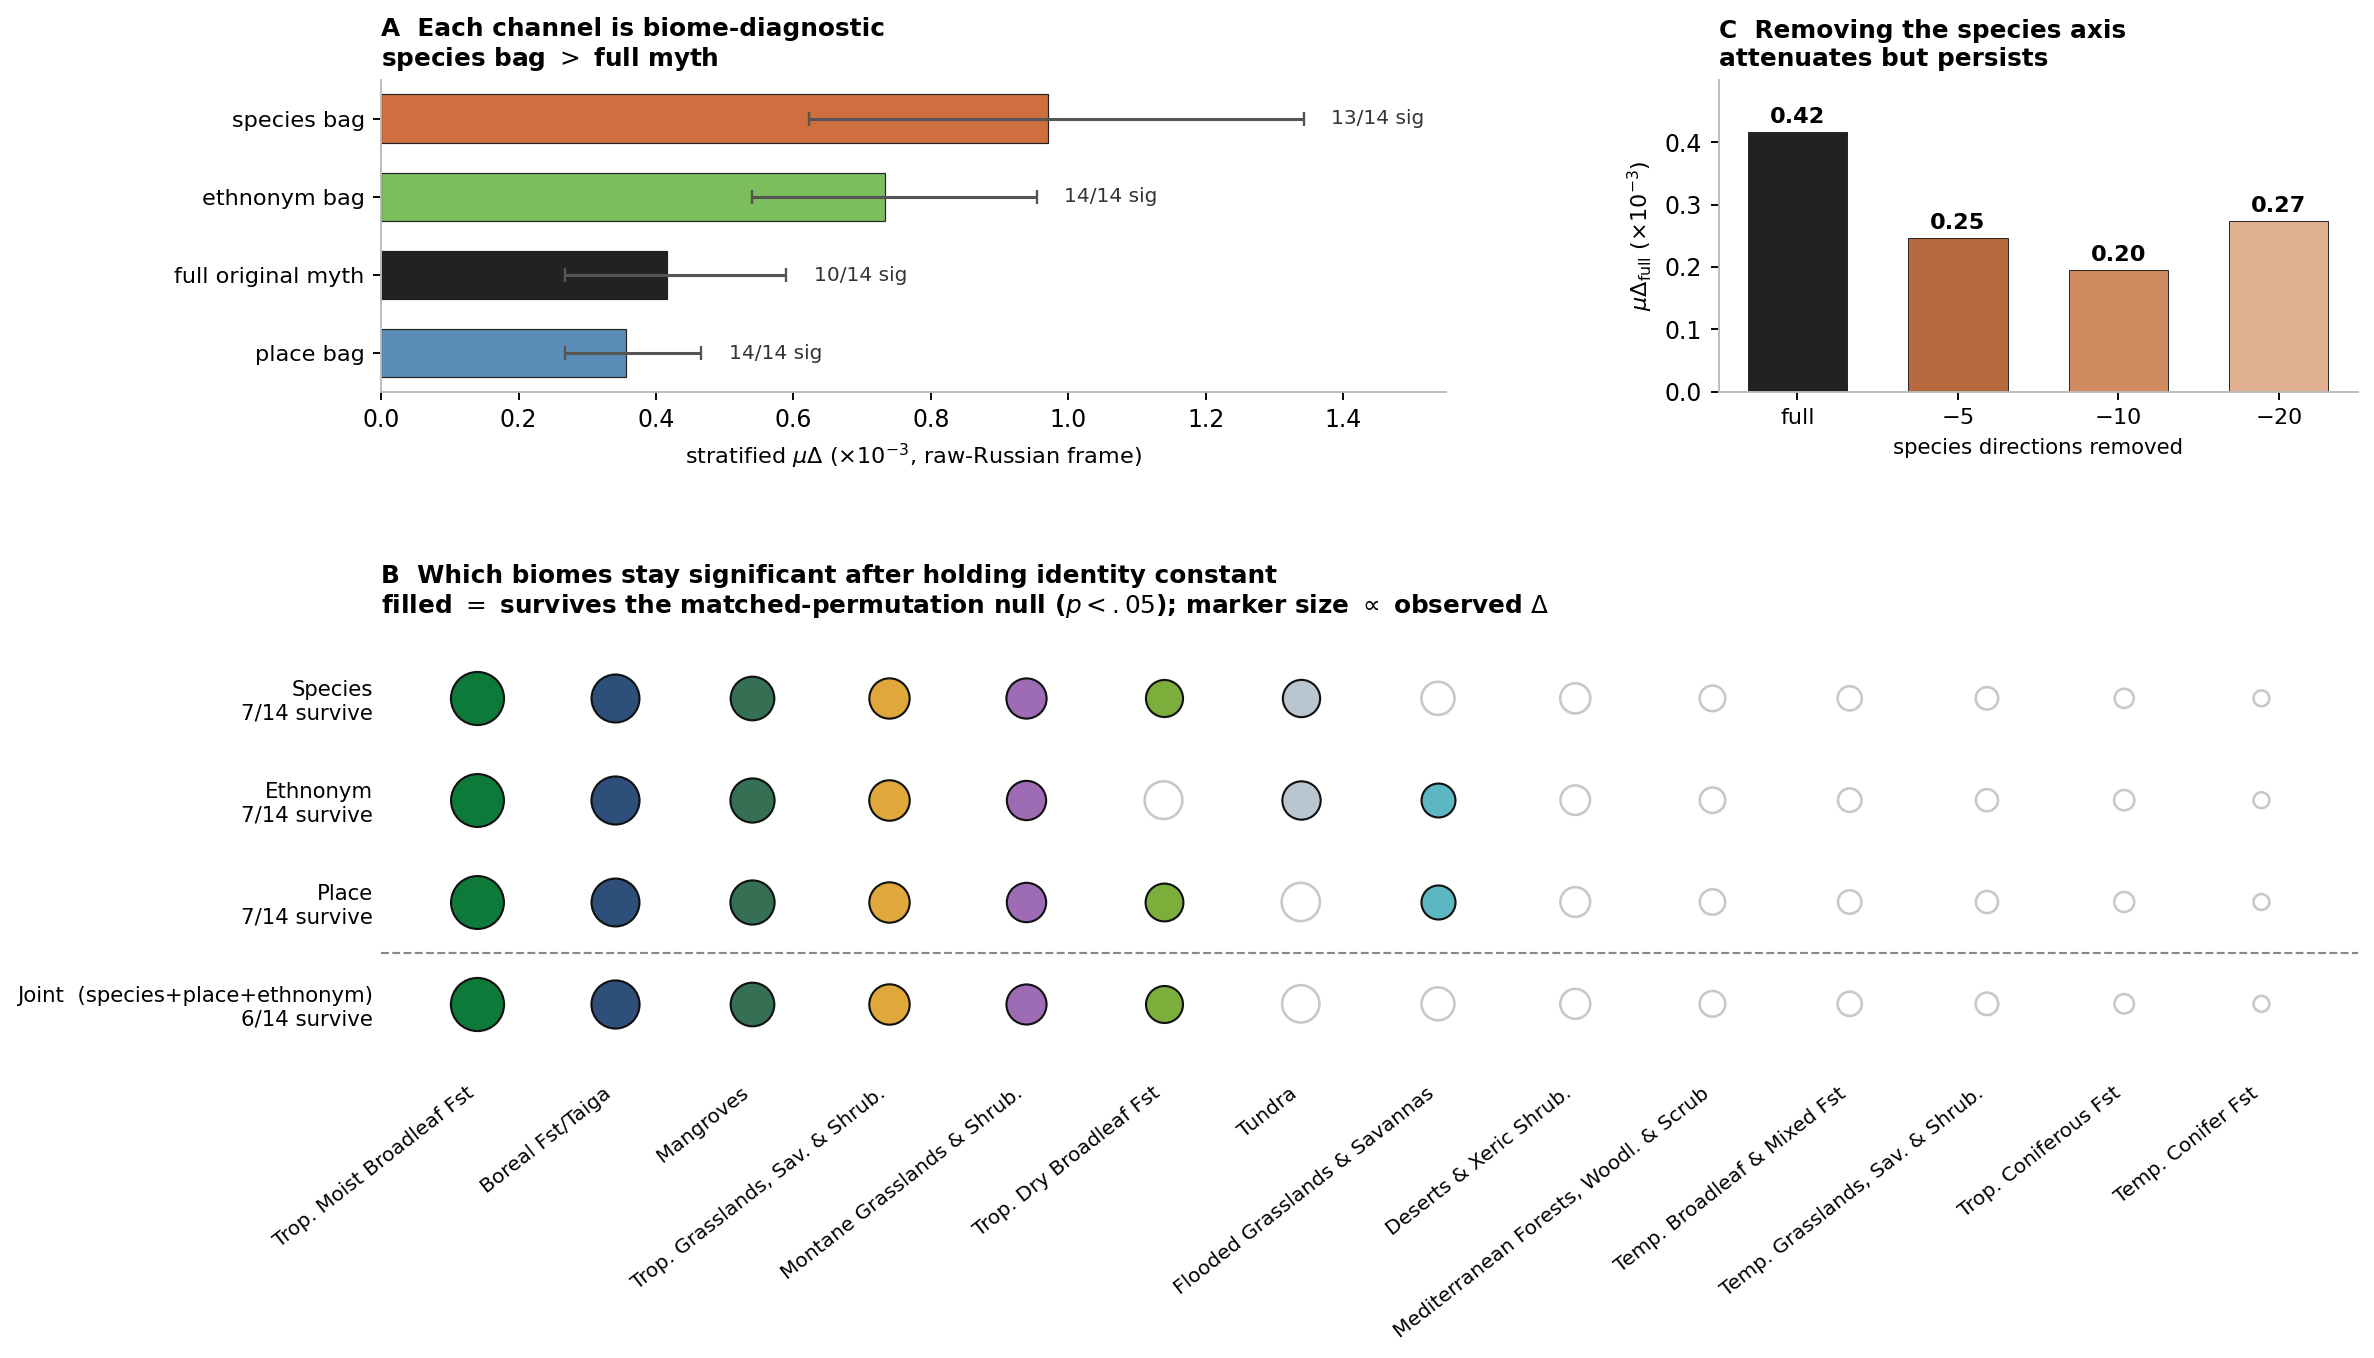
\includegraphics[width=\textwidth]{fig_identity_naming.png}
\caption{\textbf{The alignment on the original, un-anonymised myths
is not reducible to identity naming.} All panels use the
within-iconic-taxon stratified $\Delta$ in the raw-Russian frame
against iNaturalist images. \emph{Panel A}: mean $\Delta$ across
the 14 biomes (with $95\%$ bootstrap CI and the count of
individually significant biomes) for the full original myth and
three separately-measured identity baselines (species, place,
ethnonym bags). A species-only bag is more biome-diagnostic than
the full myth, and this survives stratification. \emph{Panel B}:
per-biome significance under each matched-permutation null. For
each identity class, and for all three jointly, biome labels are
shuffled only among motifs matched on that class's identity-bag
embedding ($60$ K-means blocks); a filled marker means the biome's
observed stratified $\Delta$ exceeds that null at Benjamini--Hochberg
FDR $q<.05$, an open marker that it does not, and marker size is
proportional to the observed $\Delta$. Six biomes --- Tropical Moist and Tropical Dry
Broadleaf Forests, tropical grasslands and savannas, montane
grasslands, boreal forest, and mangroves --- survive the joint null that holds
species, place, and ethnonym constant simultaneously, and five of
these survive every single-channel control. The place null is
near-circular because biome is derived from the region metadata.
\emph{Panel C}: independent embedding-space control --- the top $k$
species-subspace directions are projected out of the full-myth
embeddings and the stratified $\Delta$ recomputed ($k = 5, 10, 20$);
$\mu\Delta$ attenuates but stays positive and significant in the
majority of biomes.}
\label{fig:fig-identity}
\end{figure}

\subsection*{Breadth gradient}

\begin{figure}[h!t]
\centering
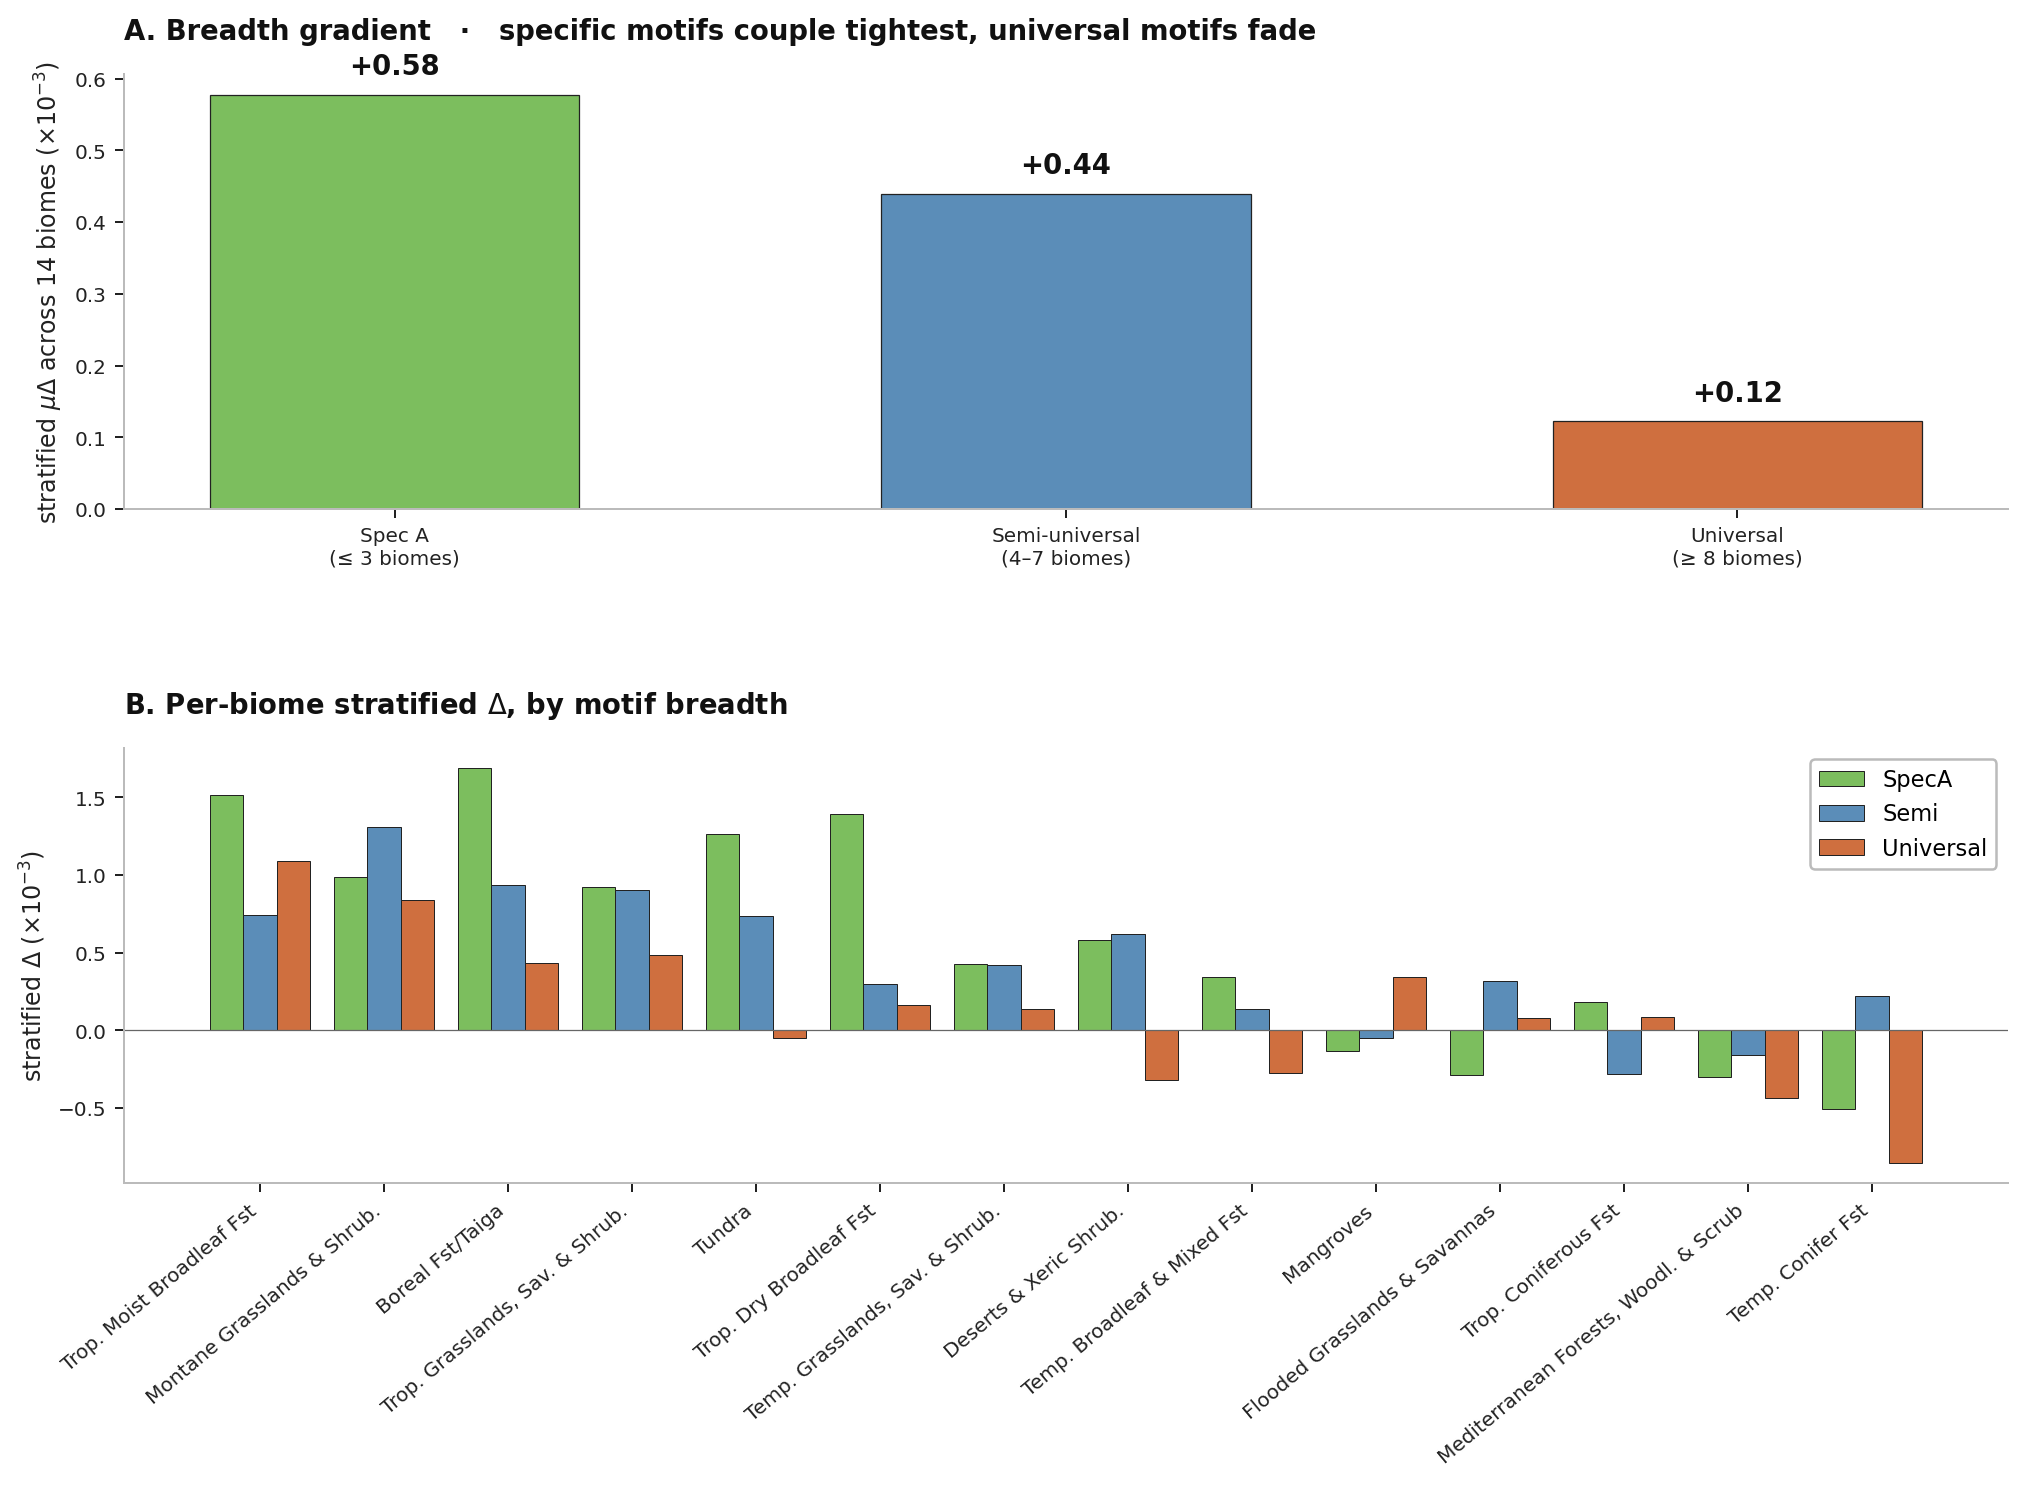
\includegraphics[width=\textwidth]{fig11_universals_analysis.png}
\caption{\textbf{Breadth-stratified analysis.} \emph{Panel A}:
across-biomes mean within-iconic-taxon stratified $\Delta$ on
iNaturalist, partitioned by motif breadth into three groups
(Spec~A: motifs touching $\leq 3$ biomes; semi-universal: 4--7
biomes; universal: $\geq 8$ biomes). The stratified $\mu\Delta$
decays monotonically from $+0.58\times 10^{-3}$ (Spec~A) through
$+0.44\times 10^{-3}$ (semi-universal) to $+0.12\times 10^{-3}$
(universal); the marginal $\Delta$ declines in parallel
($+0.52 \to +0.26 \to +0.05\times 10^{-3}$, reported in the text).
This is the pattern most naturally expected if local ecological
affordances contribute to motif stabilisation. \emph{Panel B}: per-biome stratified $\Delta$ within
each breadth group, with biomes ordered by mean stratified
$\Delta$ across the three groups. Spec~A bars (green) systematically
dominate at the high-$\Delta$ biomes (Tropical Moist Broadleaf,
Boreal/Taiga, Tropical Grasslands, Tundra, Tropical Dry Broadleaf);
universal bars (red) systematically lie at or below zero across
most biomes.}
\label{fig:fig11univ}
\end{figure}

The breadth-stratified analysis in
Figure~\ref{fig:fig11univ} provides the single test that most
informatively distinguishes the two accounts. A view in which
biome supplies only interchangeable narrative material would
expect roughly similar per-biome alignment magnitudes for
biome-specific and universal motifs, since both are equally
available as cultural projections of biome-correlated style. A
view in which local ecological affordances contribute to motif
stabilisation would expect biome-specific motifs to be the stable
points of encounter with their biome's visual structure, with
universals having propagated precisely because they detached from
any specific biome and stabilised on cross-cultural structures
(family conflict, lost-then-found, transformation). The
breadth-split result moves cleanly in the second direction. Marginal $\mu\Delta$ decays from $+0.52\times
10^{-3}$ on Spec~A motifs through $+0.26\times 10^{-3}$ on
semi-universals to $+0.05\times 10^{-3}$ on universals; stratified
$\mu\Delta$ decays from $+0.58\times 10^{-3}$ through $+0.44\times
10^{-3}$ to $+0.12\times 10^{-3}$. Five of fourteen Spec~A
biome cells are individually significant under within-taxon
stratification, against seven of fourteen for semi-universals and
two of fourteen for universals; the Spec~A subset carries a much
larger per-biome effect with proportionally similar significance
density. The signature is present where an ecological-affordance reading
would locate it, attenuated where breadth dilutes the
environmental tie, and essentially absent where motifs have
propagated across $\geq 8$ biomes.

A text-property alternative could in principle produce this
gradient without any ecological decoupling, since universal motifs
are longer and more abstract --- here breadth correlates with
motif length at $r=+0.27$ --- so a more diffuse, less
biome-lexical text might simply yield a smaller $\Delta$.
Recomputing the gradient within motif-length terciles rules this
out for the bulk of the corpus: the decline from biome-specific to
universal motifs persists within the short and mid-length terciles
(short, $+0.59 \to +0.42 \to +0.13\times 10^{-3}$; mid,
$+0.94 \to +0.27 \to +0.03$), where length is held approximately
constant and cannot drive it. The gradient does interact with
length, flattening and reversing within the longest tercile
($+0.48 \to +0.51 \to +0.60$, where long universal narratives
accumulate enough biome-relevant content to align), so it is best
read as a property of the shorter, more biome-anchored motifs
rather than a uniform law. The length-control script is released
with the code.

\subsection*{Per-taxon decomposition}

\begin{figure}[h!t]
\centering
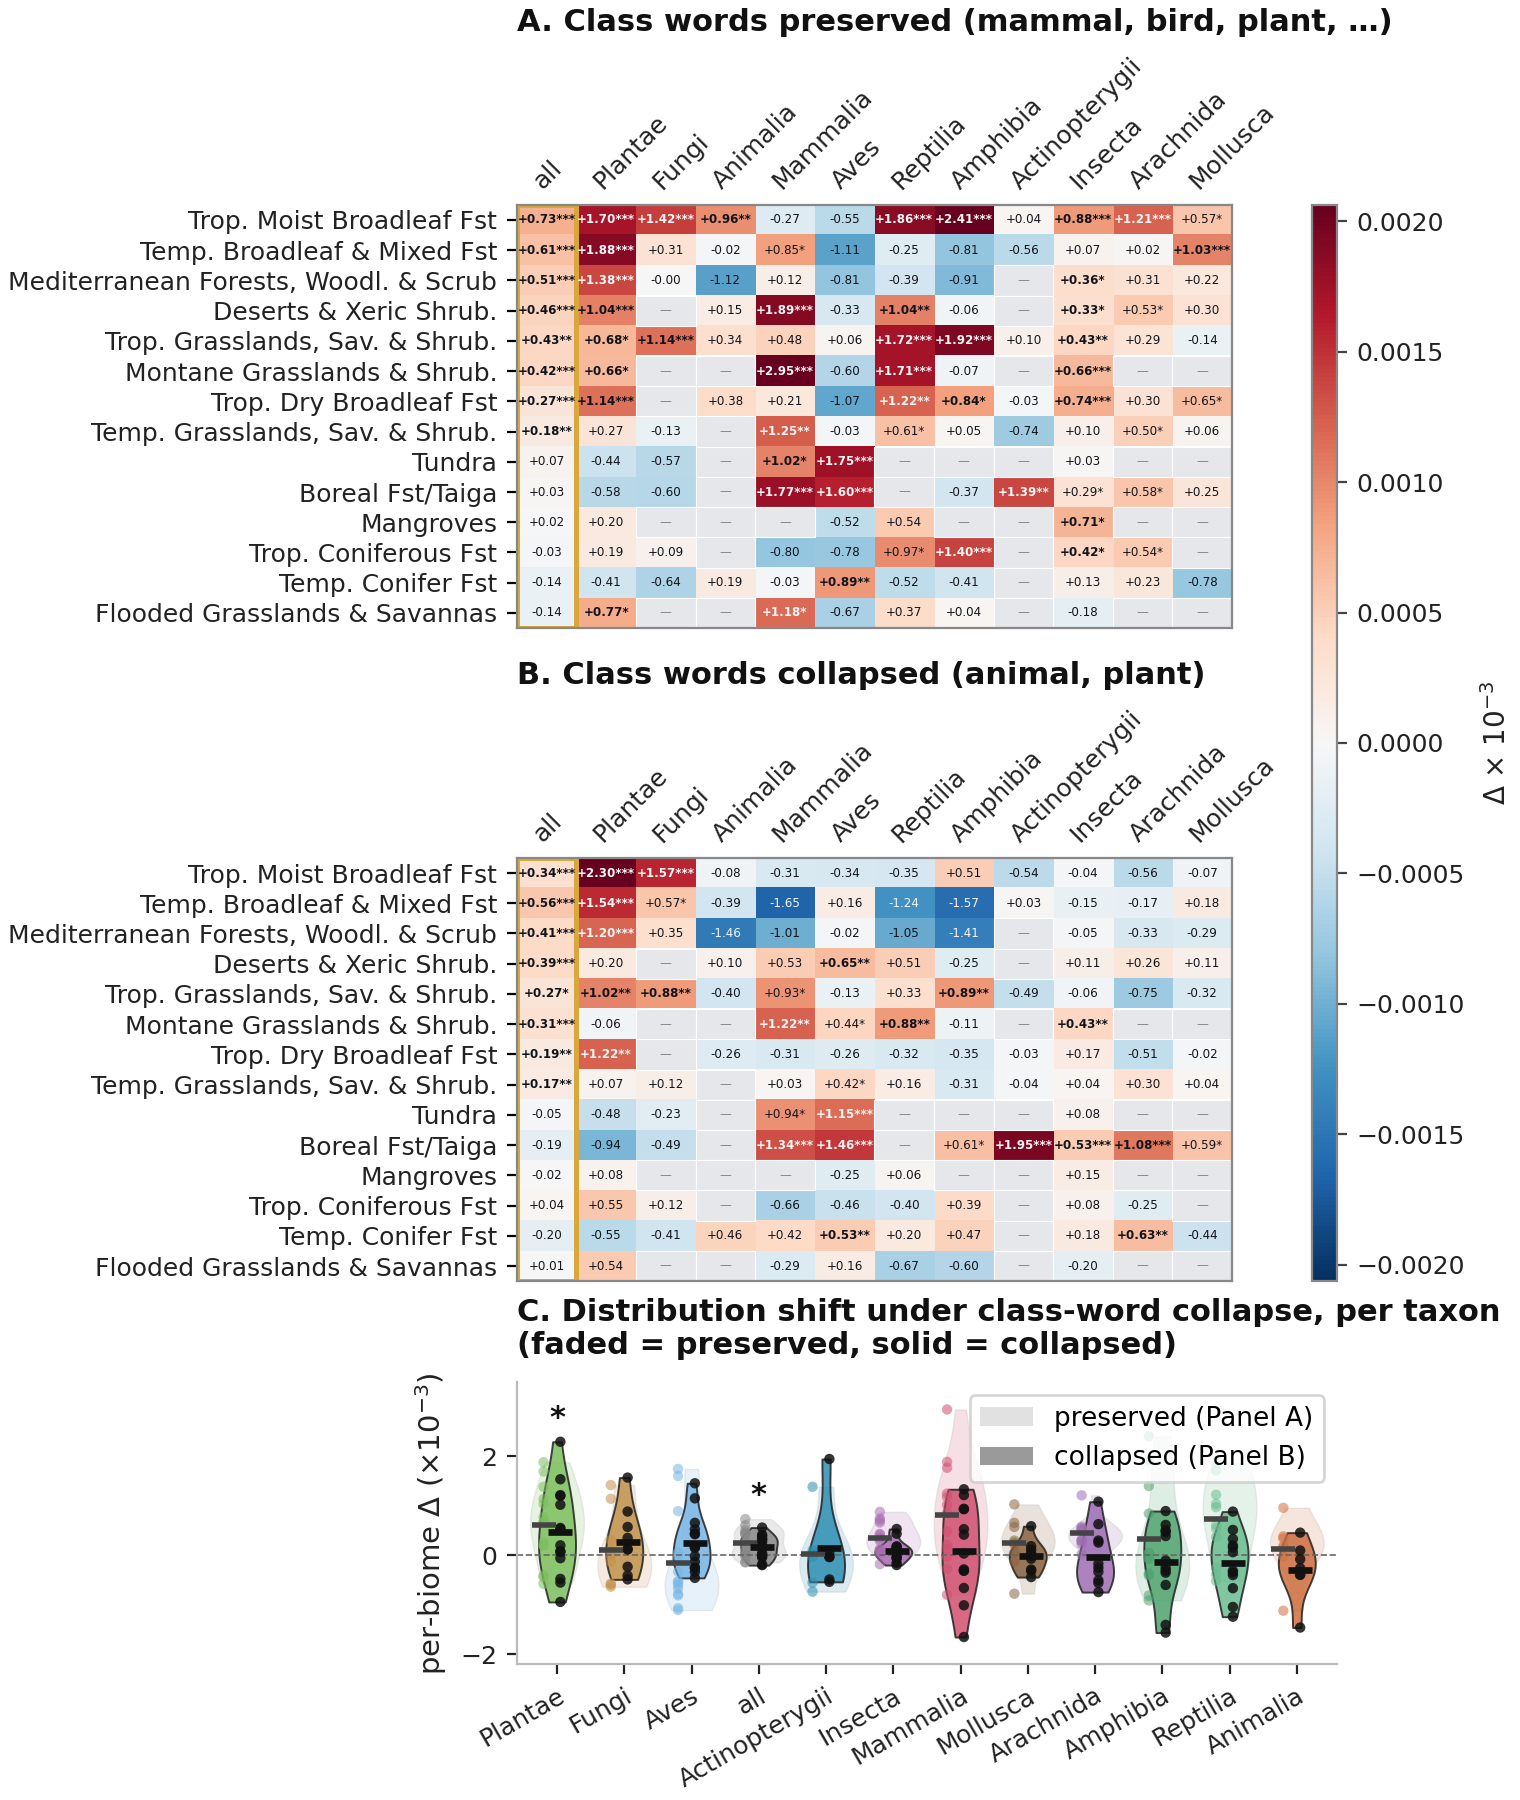
\includegraphics[width=\textwidth]{fig_taxon_combined.png}
\caption{\textbf{Per-taxon decomposition with class-word collapse
control.} Biome $\times$ iconic-taxon residualised $\Delta$ on
sentence-pooled SigLIP-2 over the full LLM-clean corpus.
\emph{Panel A:} class words preserved -- every specific species
name has been replaced by its class word (\texttt{mammal} /
\texttt{bird} / \texttt{fish} / \texttt{tree} / \texttt{plant},
etc.) but the class words remain distinct. \emph{Panel B:} class
words collapsed -- every animal-kingdom class word further reduced
to the single token \texttt{animal} and every plant-kingdom word
to \texttt{plant}, so class-word frequency is identical across
biomes by construction. Rows are the 14 WWF biomes, ordered by
descending pooled (\texttt{all}) $\Delta$ in Panel A. Cell values
are per-biome per-taxon $\Delta$ in $\times 10^{-3}$, with stars
for nominal significance and bold for BH-$q < 0.05$ within the
taxon. Cells with fewer than 10 biome--taxon photographs are
shown as grey em-dashes. The gold-bordered \texttt{all} column
anchors the marginal headline. \emph{Panel C:} for each taxon, a
double-violin contrasts the distribution of its 14 biome cells
under the two encodings -- faded behind for Panel A, solid in
front for Panel B. Taxa are ordered left-to-right by descending
collapsed mean $\mu_C$. Mean markers and per-taxon Wilcoxon
p-values (against $\Delta = 0$) appear beneath. Plantae, Fungi,
Aves, and Insecta retain most of their across-biome alignment
under collapse, indicating that the per-(biome, taxon) coupling
for those taxa is carried by surrounding lexical-thematic content
(activities, landform vocabulary, narrative shape) rather than by
the class word alone. Mammalia, Reptilia, and Amphibia attenuate
substantially, indicating that a large part of their preserved-
encoding signal was class-word frequency mirroring image-class
frequency.}
\label{fig:fig10}
\end{figure}

The per-taxon decomposition reports the per-cell \emph{marginal}
$\Delta$ within each biome--taxon stratum. Because each cell is
already conditioned on a single iconic taxon, no further taxon
stratification applies within the cell, and the headline
within-iconic-taxon stratified $\Delta$ on iNaturalist reported
in Figure~\ref{fig:fig2} is mechanically the uniform mean of
these per-cell marginal values across taxa. The matrix is
therefore not a separate analysis from the headline but its
building blocks.

Reading the per-biome × per-taxon matrix (Figure~\ref{fig:fig10},
Panel A) row by row reveals that every biome's strongest cells
fall in the taxa ecologically characteristic of it. Boreal
Forests/Taiga is carried by Mammalia, Aves, and Actinopterygii
(bears, owls, salmon); Tundra by Mammalia and Aves; Montane
Grasslands by Mammalia, Reptilia, and Insecta; the wet tropics
(Tropical Moist Broadleaf, Tropical Grasslands \& Savannas) by
Reptilia, Amphibia, Plantae, and Fungi; Mediterranean Forests
almost exclusively by Plantae; Deserts \& Xeric Shrublands by
Mammalia, Plantae, and Reptilia. The alignment is not
concentrated in any single class but distributes across the
per-biome ecologically appropriate fauna and flora.

A trivial reading of this matrix is that the class words
themselves are doing the work. Biome b's photos contain biome
b's characteristic fauna, biome b's anonymised motif text
references those fauna by class word (``mammal'' more often in
boreal mythology, ``reptile'' more often in tropical mythology)
because biome b's mythology grew up around those animals, SigLIP
notices the alignment as a class-word-frequency artefact, and the
cells are positive by simple co-occurrence. The class-word
collapse control in Panel B tests this directly. We re-embedded
the same LLM-clean corpus after collapsing every animal-kingdom
class word (mammal, bird, fish, reptile, amphibian, insect,
mollusc, crustacean, arachnid) to the single token ``animal'' and
every plant-kingdom word (tree, flower, plant, fungus) to
``plant''. Class-word frequency is now constant across biomes by
construction. Every animal mention reads ``animal'', every plant
mention reads ``plant'', no biome's text carries any class-word
information beyond ``some animal'' or ``some plant''.

The result is informative on both sides. The pooled alignment
attenuates by about a third (the \texttt{all} column $\mu\Delta$
drops from $+0.244\times 10^{-3}$ to $+0.160\times 10^{-3}$, with
the matrix retaining a per-cell Pearson $r = +0.57$ against its
class-word-preserved counterpart). Per-taxon means change
substantially for the vertebrate animal classes: Mammalia falls
from $+0.82$ to $+0.09 \times 10^{-3}$, Reptilia from $+0.74$ to
$-0.16$, Amphibia from $+0.33$ to $-0.14$. Plant content is more
robust: Plantae drops only from $+0.61$ to $+0.48 \times 10^{-3}$.
A substantial component of the per-(biome, taxon) signal for
animals \emph{was} class-word frequency mirroring image-class
frequency. But the pooled effect does not collapse to zero, and
the biomes whose cells stay strongly positive under the collapse
(Tropical Moist Broadleaf, Temperate Broadleaf, Mediterranean
Forests on Plantae and Fungi; Boreal Forests/Taiga and Tropical
Coniferous Forests on Insecta and Mollusca) tell us where the
coupling is carried by content beyond the class word.

The collapse therefore partitions the per-taxon alignment into
two components. For animal classes, the class word itself
accounts for most of the per-cell work, and the residue after
collapse is small. For plant and fungus classes, the alignment
was carried from the start by something other than the class
word, and that something survives the collapse largely intact.
The Kruskal--Wallis omnibus across taxa under either encoding is
not significant, and no individual taxon survives BH correction
at the taxon level; with only 14 biome cells per taxon, the test
has limited power to discriminate distributions across taxa and
we do not claim a statistical separation between them.

Three components of the biome--mythology alignment can therefore
be distinguished on the basis of the collapse. First, a weaker
class-frequency ecological signal in which biome-$b$'s text
mentions a given class word more often because biome-$b$
mythology is built around that class; the encoder reads the
overlap from the names alone. This component is concentrated in
the vertebrate animal taxa (Mammalia, Reptilia, Amphibia) and
dissolves under the collapse. Second, a stronger residual
lexical-thematic signal carried by the activities and narrative
context the motif text builds around its biome's flora and
fauna; this component is concentrated in the plant- and
fungus-coded cells and survives the collapse largely intact.
Third, the broader biome-level signal reported in
Figure~\ref{fig:fig2}, which combines both contributions because
the stratified per-biome $\Delta$ is the uniform mean of the
per-(biome, taxon) cells from which both components originate.
The conservative version of the biome-level coupling claim
therefore runs through the second component, the part that
survives the class-word collapse. We unpack what this asymmetry
suggests about how mythology engages different parts of the
biome in the Discussion.

\subsection*{Biome structure is recoverable without supervision}

The analyses so far compare each motif to images grouped by a
biome label we supply. As a converging check that never uses biome
labels to build the representation, we re-described every motif by
its \emph{affinity profile}: the vector of its residualised cosine
similarities to all $46{,}481$ iNaturalist photographs (per-motif
centred, as in the headline $\Delta$). Two motifs are neighbours in
this space when the same images draw them in and push them away,
whatever those images depict. An unsupervised embedding of the
geometry (PCA to 50 dimensions, then UMAP) is organised first by
depicted \emph{content}: colouring the map by each motif's dominant
taxon recovers more structure (adjusted Rand index $0.08$) than
colouring it by cultural macro-area ($0.04$) or by biome ($0.02$).
The geometry is dominated by what the myths are about rather than
where they are from, and a biome-coloured scatter shows no clean
clustering.

Biome is nonetheless present as a subdominant but reliable overlay,
recoverable two ways without ever using biome labels to construct
the affinity vectors (Figure~\ref{fig:fig-recovery}). First, for
each motif we ranked the nine well-sampled biomes by the motif's
taxon-stratified mean similarity to their images and asked where
the motif's own biome fell. Own biome lands at the $64$th
percentile on average against a $50$th-percentile chance baseline
($p<.001$, $2{,}000$ label permutations; Figure~\ref{fig:fig-recovery}A).
Second, a
five-fold one-versus-rest logistic probe on the PCA-reduced
affinity vectors decodes each biome above its label-shuffled null,
at a mean balanced accuracy of $0.66$ against $0.50$
(Figure~\ref{fig:fig-recovery}B). The affinity vectors are built
from the anonymised text, in which species names are already class
words, and both diagnostics are essentially unchanged when the text
is collapsed further so that every animal class reads only
``animal'' and every plant class only ``plant'' (retrieval
percentile $0.63$, decodability $0.66$ against a $0.50$ null), so
the recovered biome structure is not the species or taxon channel
but the lexical-thematic content around it. The biome signal is
real and recoverable from the model's image affinities alone, but
it is a thin overlay on a geometry that is otherwise organised by
the kinds of plants, animals, and scenes the myths describe.

\begin{figure}[h!t]
\centering
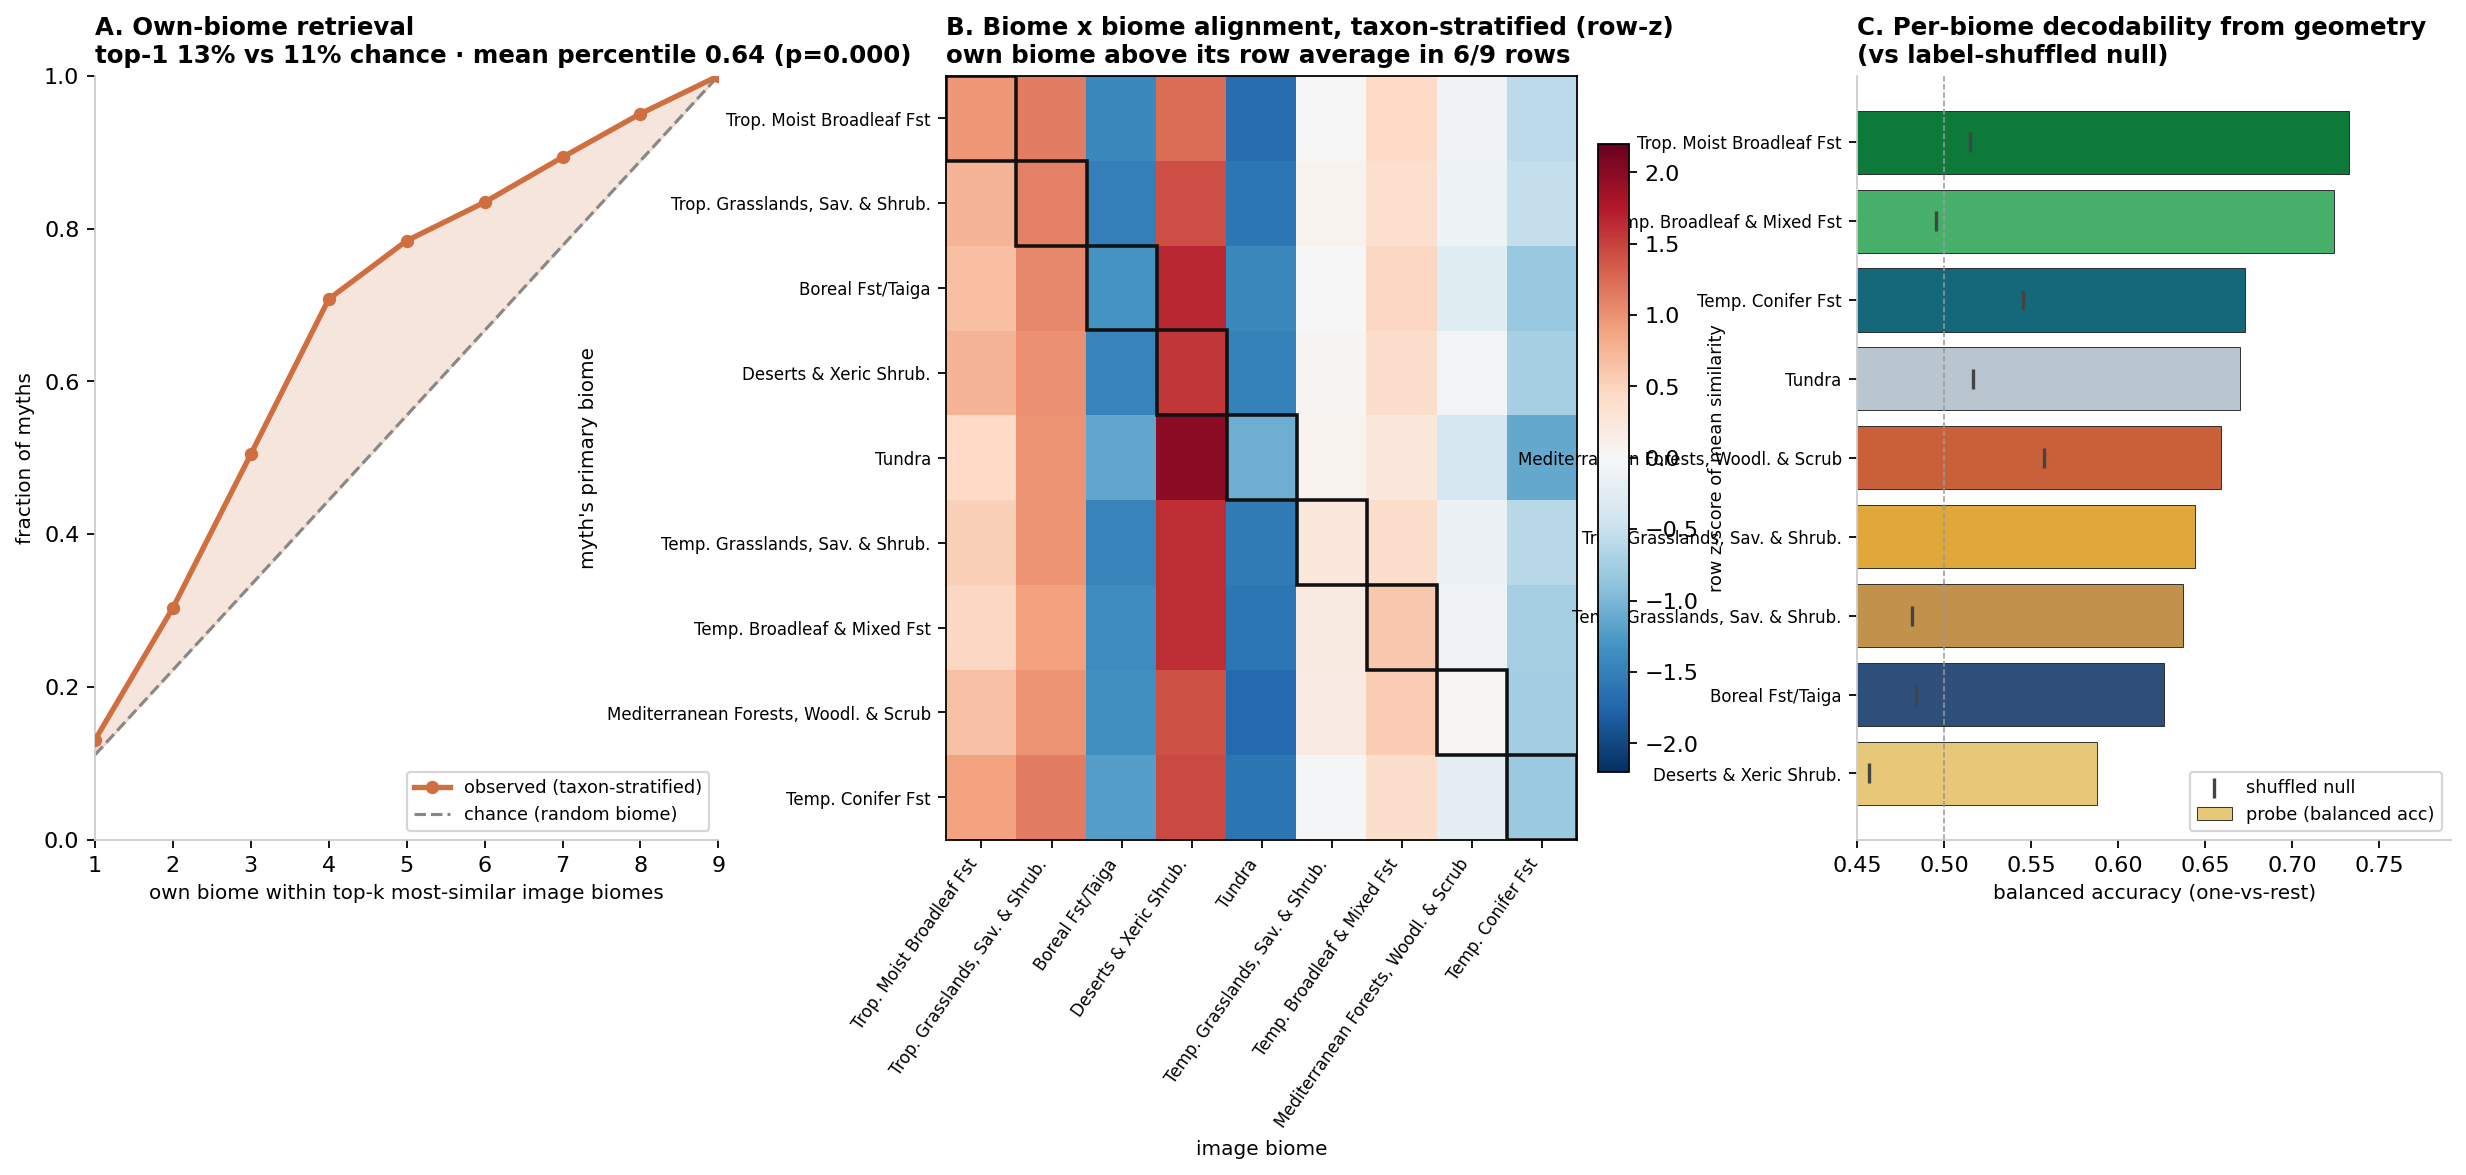
\includegraphics[width=\textwidth]{fig_biome_recovery.png}
\caption{\textbf{Biome structure is recoverable from the
unsupervised myth--image affinity geometry, without using biome
labels.} Each motif is represented by its residualised
cosine-similarity profile across all $46{,}481$ iNaturalist
photographs. \textbf{(A)}~Own-biome retrieval. For each motif the
nine well-sampled biomes are ranked by the motif's taxon-stratified
mean similarity to their images; the curve gives the fraction of
motifs whose own biome falls within the top $k$ ranks (orange)
against the chance diagonal (grey). Own biome reaches the $64$th
percentile on average ($p<.001$, $2{,}000$ permutations).
\textbf{(B)}~Per-biome decodability. Balanced accuracy of a
five-fold one-versus-rest logistic probe on the PCA-50 affinity
vectors (bars) against a $200$-shuffle label-permuted null (mean
$\pm 2$ sd); all nine biomes decode above chance at
Benjamini--Hochberg FDR $q<.05$, at a mean of $0.66$ versus $0.50$.
Throughout, ``own biome'' is the biome contributing the most of a
motif's traditions, and the affinity vectors are built without
reference to it.}
\label{fig:fig-recovery}
\end{figure}

% =============================================================================
\section*{Discussion}

The mythologies of nearly a thousand cultures, stripped of every
species name, place name, biome word, and ethnonym we could
identify, still align preferentially with images of the biomes
those cultures inhabit. The alignment holds on two independent
visual corpora, replicates across four vision--language models,
and decays monotonically as motifs propagate beyond their biome of
origin: tightest where the mythology is biome-specific, fading to
nearly nothing where it has spread to most of the world. We read
this pattern as evidence that mythology carries, in the
lexical-thematic structure of its surviving text, a recoverable
residue of the perceptual encounter between culture and biome.

\subsection*{Mythology as a recording layer of perceptual coupling}

The breadth gradient is the result that most informatively
distinguishes the two accounts of mythology we set out to test. A
view in which mythology's symbolic content is largely a function
of mind and culture and the environment supplies raw material but
not form has no principled reason to expect that biome-specific
motifs and universal motifs should align with their biomes'
imagery at different rates. The two classes of motif are equally
available as projection surfaces under that reading. A coupling
reading accommodates the gradient more naturally. Biome-specific
motifs are, on this account, the stable points of an encounter
between a culture and a particular ecology, and their
lexical-thematic content was shaped in that encounter. Universal
motifs propagated precisely because they detached from any single
biome and stabilised on cross-cultural structures (family
conflict, transformation, the journey to and from the dead)
whose conditions for stabilisation are not ecological. Universals
fade because the coupling has been factored out of them.

That reading converts mythology, in the technical sense, into a
\emph{recording layer}: not a description of the biome, and not a
projection onto it, but a residue of the work the biome did in
shaping which narrative completions were ecologically reinforced
and which were not. The motif catalogues of computational
mythography~\citep{berezkin2024catalogue,thuillard2018folktale,tehrani2013phylogeny}
are, on this view, partial transcripts of a process that runs
across many human generations and is irreducible to either side
of the perceiver--environment pair. The phylogenetic mythology
program~\citep{tehrani2013phylogeny,daribigne2017phylogenetic} has
shown that motifs can be tracked across cultural genealogies as
faithfully as genes; the breadth gradient we observe adds a
complementary claim, that within those genealogies the motifs
that stay tied to a single biome are the ones whose ecological
substrate kept selecting for the same coupling, while the motifs
that spread are the ones whose stabilisation was no longer
biome-dependent.

\subsection*{A cognitive ecology of imagination}

The lineage that makes this reading philosophically articulate
runs across two centuries. Schelling's distinction between
\emph{natura naturata} (nature as finished product) and
\emph{natura naturans} (nature as productive activity becoming
aware of itself)~\citep{schelling1797ideas,schelling1799outline}
was recovered in the twentieth century by
Bateson~\citep{bateson1972steps,bateson1979mind}, who turned it
into a cybernetic claim: mind is wherever the conditions for a
mental process obtain, wherever differences make differences,
wherever pattern propagates across coupled systems. A human
imagining a figure in a cliff face is not generating an inner
image and applying it to outer matter. The imagining is an event
in a coupled system that includes neural pattern-completion
machinery, the actual statistical structure of the cliff, the
cultural priors that have shaped what counts as a figure to be
found, and the linguistic apparatus that will or will not
stabilise the percept into a transmissible name. Pull any element
from the system and the event does not occur, or occurs
differently. Depth psychology developed a parallel challenge to
projection: Jung's mature view located the archetypes in the joint
between psyche and nature rather than in either
alone~\citep{jung1959archetypes}; Hillman read imagination as
responsive, finding figures already there to be
found~\citep{hillman1975revisioning,hillman1981thought}; Corbin
named the \emph{mundus imaginalis}, a domain of real forms
encountered through trained imagination and distinct from the
modern collapse of ``imaginary'' into ``merely
subjective''~\citep{corbin1972mundus,abram1996spell}. Ingold's
ecological anthropology generalised the move beyond personhood:
human life is \emph{dwelling}, not the projection of cultural
schemes onto an external world but ongoing participation in a
field of relations that produces both the dweller and the
dwelt-in~\citep{ingold2000perception,descola2013beyond}.

The cognitive sciences, beginning with Gibson's ecological
psychology~\citep{gibson1979ecological} and generalised by the 4E
program (embodied, embedded, extended, and enactive cognition)
~\citep{varela1991embodied,clark1998extended,noe2004action},
supplied the empirical scaffolding. Predictive processing gave
the mechanism: the brain as a hierarchical prediction machine
locking onto interpretations its priors privilege, given the
actual statistical structure of what the world
presents~\citep{friston2010free,clark2016surfing,hohwy2013predictive}.
Niche construction theory closed the
loop~\citep{odlingsmee2003niche}: humans produce symbolic
environments (names, stories, transmitted schemas) and those
environments in turn shape the cognition of subsequent
generations. On this synthesis, a figure in a biome is the stable
point of a three-way coupling between environmental structure,
perceptual machinery, and cultural transmission; imagination is
not a private generative act but the moment of stabilisation in
that coupling; and mythology is the cultural recording layer that
keeps the stabilised completions available across generations.

The result reported here is more naturally accommodated by a
coupling or ecological-affordance account than by a view in
which biome supplies only interchangeable narrative material. A
vision--language model is a system without perceptual
phenomenology, without cultural participation, and without
priors shaped by deep evolutionary time. That such a system,
trained on the public products of the coupling, recovers the
coupling's signature in the joint statistical structure of
environments and the stories told within them is what one would
expect if the structure is really there to recover. It is, in
Bateson's vocabulary, a difference that makes a difference at
the joint, detectable from either side.

\subsection*{What kind of coupling: the lexical-thematic level}

A coupling claim has to be carried at some level of the text.
Our analyses locate it at the lexical-thematic level rather than
at the level of narrative structure. The alignment survives
word-shuffling of each motif, so sentence-level composition is
not where the residue lives; it disappears on synthetic
encyclopedic paragraphs, so the residualised statistic does not
manufacture a positive on biome-neutral content (both in
Supplementary Section~S1, Figure~\ref{fig:v2controls}); and it
persists in motifs whose anonymised text alone provides minimal
text-only biome predictability, so it is not reducible to a
one-sided lexical artefact (Supplementary
Section~\ref{sec:biome-tell}, Table~\ref{tab:biome-tell-split}). What is doing the work, in other words, is the
distribution of generic landform vocabulary and biome-correlated
activity schemas that the noun-targeted anonymisation pipeline
retained by construction.

This level is the one a strict perceptual-coupling reading
predicts. Activities (gathering, hunting, fishing, herding,
fording, climbing) are not free parameters of culture overlaid on
an inert environment; they are biome-constrained possibilities,
the affordances Gibson named, that the environment makes
available to the perceiver. Generic landform words (forest,
mountain, river, snow, sand, sea) are not biome labels but the
articulated joints of the perceived world, the structural
features around which attention and narrative
organise~\citep{ingold2000perception,descola2013beyond}. A
mythology that stabilises around the affordances and
articulations of its biome is not failing to be symbolic; it is
recording, in the only medium it has, the schemas of attention
that the biome made available. The breadth gradient predicts that
universals should be precisely the motifs whose stabilisation
required affordances common to most environments, and that is
what we find.

This is also the move that rescues the result from being merely
methodological. The two-corpus replication is informative here.
Activity vocabulary in the cleaned text could in principle align
with activity \emph{photographs} on a corpus that contained them.
Places365's strict-landscape filter removes humans, vehicles,
and depictions of activity, leaving only terrain and vegetation,
and the alignment persists with comparable magnitude on that
corpus. That is the signature of a coupling whose residue is
read at the morphological level of the scene, not at the level of
matching activity descriptions to activity images. The per-taxon decomposition makes a more careful version of the
parallel argument from the species side, and what it shows is an
asymmetry between the two kingdoms. The class-word collapse
splits the per-(biome, taxon) signal into the part the encoder
reads from the class word alone and the part carried by the
surrounding lexical-thematic content. For animal-coded biomes
the class word does most of the per-cell work. Boreal mythology
references ``mammal'' more often because boreal mythology is
full of bears and wolves; iNaturalist boreal photographs contain
mammals because the boreal contains mammals; the encoder reads
the overlap from the names alone. When the animal class words
are collapsed to a single ``animal'' token, the Mammalia,
Reptilia, and Amphibia cells deflate substantially because the
alignment lived in the naming layer. For plant-coded and
fungus-coded biomes the asymmetry reverses. Plant naming in
mythology is thin to begin with; most plants in the catalogue
are already just ``plant'' or ``tree'' even before any further
collapse, so the per-cell alignment had to come from something
else from the start. The activities mythology built around
plants (fruit-gathering, sacred groves, orchard-tending,
vine-cultivation, the narrative roles plants take as origins,
gifts, and transformations) are what align with the visual
structure of biome-$b$'s actual flora in their habitat, and
they have nowhere else to go when the class word is removed.
Plantae and Fungi cells survive the collapse with most of their
magnitude intact across precisely the biomes where mythology
engages local flora most thickly.

That asymmetry suggests two different modes of mythological
engagement with the biome. Some inhabitants get named, walking
through stories under their class identity --- the mammals,
reptiles, and amphibians whose vocabulary trace the encoder
reads trivially. Others get encountered, narrated around, and
stabilised through their roles in transformation, journey, and
dwelling --- the plants, fungi, birds, and insects whose
mythological presence is built more from activities and contexts
than from names. The class-word collapse separates these two
modes and shows that both are real. The conservative version of
the coupling claim runs through the second, where it can be most
cleanly tested because the vocabulary that would carry a trivial
alignment has been emptied out. That biome-$b$'s plants and fungi
still align with biome-$b$'s mythology when the text says only
``plant'' is the cleanest single demonstration that mythology
records something of its biome beyond the names of what lives
there.

The anonymisation pipeline and the class-word collapse both make
this point by \emph{removing} naming from the text. The
identity-naming analysis (Figure~\ref{fig:fig-identity}) reaches
the same conclusion from the opposite direction, keeping the
original myths intact and instead holding the species, place, and
ethnonym channels constant statistically on the same stratified
statistic. On that statistic the un-anonymised full myth aligns
almost exactly as strongly as the anonymised one, and a bag of
species names is more biome-diagnostic than the full myth, yet the
alignment still persists in roughly half the biomes once all three
naming channels are held constant and under a projection that
removes the species axis from the embeddings. The two strategies
rest on assumptions that do not overlap --- one trusts the
cleaning and removes the taxon confound, the other trusts no
cleaning and removes the confound through stratification --- and
they converge: the biome--mythology alignment is not reducible to
the trivial channel by which a biome's mythology names that
biome's species, places, and peoples.

\subsection*{Toward a falsifiable enactivist mythography}

A philosophical reading that does not generate predictions is a
worldview, not a research programme. The coupling lineage has
historically been read as a worldview; the result reported here
makes it possible to read it as a research programme with risky
predictions. If imagination is coupling, and mythology is its
recording layer, then several things should be true that follow
naturally from this reading and are not naturally generated by a
view in which biome supplies only interchangeable narrative
material. They should be increasingly directly testable.

First, the same coupling signature should appear in
mythological \emph{visual art} more strongly than in
mythological text, because art is a more direct transcript of
the perceptual encounter and has not been compressed through the
narrative-summary bottleneck Berezkin's catalogue records. A
museum corpus is under construction. Second, the signature
should be denser in oral-narrative audio than in literary
transcription, because audio preserves more of the contextual
texture that text drops. Third, the breadth gradient should
mirror the historical distribution of subsistence ecology:
motifs that decoupled from biome should track the cultural
transmission routes (trade, migration, religious conversion) that
moved them, with their original ecological substrate fading as
they entered other biomes. Fourth, motif-conditioned visual
priors should improve scene classification on photographs of the
biomes those motifs were stabilised in, because the priors
encode information about which configurations were perceptually
salient in that biome. None of these is a tautology; each can
fail; and if mythology is doing what we suggest it is doing,
each should pass.

The honest reading of what the data show is bounded. They do not
demonstrate that nature is conscious, or that mythologies are
messages from a non-human agency, or that the strongest
metaphysical readings of the coupling lineage (Whitehead's
process metaphysics~\citep{whitehead1929process}, Goff's
panpsychism or Strawson's realistic
monism~\citep{goff2019galileo,strawson2006realistic}) are
empirically supported. They show that the joint statistical
structure of environments and the stories told within them
carries a recoverable residue of their coupled history, robust
enough that a system without phenomenology can detect it from
either side. That is a smaller claim than the strongest readings
of the lineage and a larger claim than a view in which biome
supplies only interchangeable narrative material would allow.

Berezkin's corpus is curated, Eurasian-weighted, and sparse in
several biomes (Mangroves, Flooded Grasslands, Temperate Conifer
Forests). The vision--language models we use carry the biases of
their training distributions, which the cross-model agreement
bounds but does not erase. The anonymisation pipeline is
noun-targeted; an activity-vocabulary pass that strips the
remaining biome-correlated verbs is the natural next experiment,
and we expect it to attenuate but not eliminate the signal, on
the same logic that the within-Glottolog biome-swap null
attenuated rather than eliminated it: the biome-content
information is not concentrated in any single layer of the text
but distributed across the substrate that the perceptual
encounter shaped.

Schelling wrote that ``nature should be visible Mind, and Mind
invisible Nature.'' The pattern reported here is not a
demonstration of his stronger thesis, but it is more naturally
accommodated by a coupling or ecological-affordance reading of
imagination than by a view in which biome supplies only
interchangeable narrative material. Mythology, on the reading
the data support, is one of the long instruments humans have
used to keep the coupling articulate. The work of making the
coupling reading testable has only begun.

% =============================================================================
\section*{Materials and Methods}

\subsection*{Corpus and biome assignment}

We use Yu.\ E.\ Berezkin's \emph{Analytical Catalogue of World
Mythology and Folklore}~\citep{berezkin2024catalogue}, scraped from
\texttt{ruthenia.ru} in May 2024. The catalogue provides 2{,}564 motif
entries indexed across 958 traditions; each motif has a
multi-paragraph Russian-language abstract aggregating the variants
found across the traditions that carry the motif. Tradition centroids
are joined to WWF Terrestrial
Ecoregions~\citep{olson2001terrestrial} to assign each tradition, and
through it each tradition--motif pair, to one of the 14 WWF biomes. Of
the 2{,}564 catalogue motifs, the 2{,}158 analysed throughout are those
with both a successfully scraped, anonymisable abstract and at least one
tradition geocodable to a WWF biome; the remaining $406$ lack one of
these. Most of the excluded motifs have no biome-codable tradition and
so cannot enter a biome-level statistic by construction, and the
abstract-scrape failures are indexed by motif identifier rather than by
biome, so the exclusion is not biome-targeted.

\subsection*{Image corpora}

The iNaturalist component consists of $46{,}481$ images drawn from
research-grade observations on iNaturalist Open
Data~\citep{inaturalist2024} across the 14 WWF biomes. We apply an
image-side sanity filter that drops obvious non-nature content via
SigLIP-2 zero-shot scoring against twelve negative prompts
(\emph{``a person in the photo''}, \emph{``a portrait of a human''},
\emph{``people holding something''}, \emph{``an angler holding
fish''}, \emph{``an indoor scene''}, \emph{``a kitchen or
laboratory''}, \emph{``a city skyline or street''}, \emph{``a car
or vehicle''}, \emph{``a road sign''}, \emph{``a black or
all-white image''}, \emph{``a museum specimen on a white
background''}, \emph{``a screenshot or document''}). An image is
dropped if its maximum cosine similarity to any of the twelve
negative prompts exceeds $0.08$. The threshold is lenient
(removing only obvious cases) so that species-in-habitat
close-ups and natural outdoor scenes are retained, which is the
content iNaturalist is biased toward by design. For the curated landscape comparison, the Places365
component~\citep{zhou2018places} is drawn from scene categories
whose semantic interpretation unambiguously corresponds to a
single WWF biome (e.g.\ \emph{tundra} $\to$ arctic tundra;
\emph{rainforest} $\to$ tropical moist broadleaf;
\emph{forest/broadleaf} $\to$ temperate or tropical dry
broadleaf; \emph{snowfield/mountain\_snowy} $\to$ boreal/taiga;
\emph{lagoon/swamp/creek/coast} $\to$ mangroves); categories that
mix biomes were excluded. Each candidate image is then passed
through a strict-landscape SigLIP-2 filter that drops anything
that is not a wide-shot natural scene: five positive prompts
(\emph{``a wide-shot natural landscape with no people''},
\emph{``a panoramic photograph of natural scenery''}, \emph{``an
empty natural habitat photographed from a distance''}, \emph{``a
landscape photo of natural terrain showing vegetation and
horizon''}, \emph{``a wild ecosystem with no human-made
structures''}) and eleven negative prompts (\emph{``a person in
the photograph''}, \emph{``a portrait of one or more humans''},
\emph{``a close-up photo of a single animal''}, \emph{``a single
bird filling the frame''}, \emph{``a car or vehicle''}, \emph{``a
boat''}, \emph{``a road or street''}, \emph{``a man-made structure
or building''}, \emph{``an indoor scene''}, \emph{``a person
riding a horse or animal''}, \emph{``a tourist photograph with
people''}) are encoded by SigLIP-2 and compared against each
image's embedding. The strict-landscape score is
$\mathrm{mean}(\text{positives}) - \max(\text{negatives})$; an
image is dropped if its $\max(\text{negatives}) > 0.18$, and the
remaining top-$K$ images per biome are kept. The Places365 filter
is intentionally stricter than the iNaturalist filter, in
particular it removes single-species close-ups, because the
Places365 panel functions as a scene-only robustness check on
biome-character imagery, complementary to iNaturalist's
species-in-habitat coverage.

\subsection*{Vision--language embedding}

The headline model is SigLIP-2-large
(\texttt{google/siglip2-large-patch16-384})~\citep{tschannen2024siglip2},
a multilingual vision--language model with native Russian support.
Images use the standard $384\times 384$ preprocessing. Text is
sentence-pooled: each LLM-clean Berezkin abstract is split into
sentences (regex on terminal punctuation, sentences of $<3$ words
dropped, capped at $50$ sentences per motif), each sentence is
embedded independently within SigLIP-2's $64$-token window
(mean $23$ sentences per motif; $50{,}032$ sentences in total across
$2{,}158$ motifs in total), and the per-motif vector is the
mean-pooled, L2-renormalised sentence embedding. Sentence pooling
matters because the raw English abstracts average $\sim 3{,}400$
tokens, of which a $64$-token truncation captures only the first
$\sim 2\%$; the sentence-pooling pass embeds the full anonymised
abstract instead. For cross-model robustness we additionally embed
with M-CLIP (\texttt{XLM-Roberta-Large + CLIP-ViT-L/14})~\citep{carlsson2022mclip}
on the Russian abstracts (M-CLIP's $512$-token window covers most
abstracts in a single forward pass) and with OpenCLIP-ViT-L/14
(LAION-2B and OpenAI pretrainings) on English motif oneliners
(see Supplementary Figure~\ref{fig:figS-crossmodel}). Image and
text features are L2-normalised and similarity is the inner
product.

\subsection*{Controls against biome cues}

\begin{figure}[h!t]
\centering
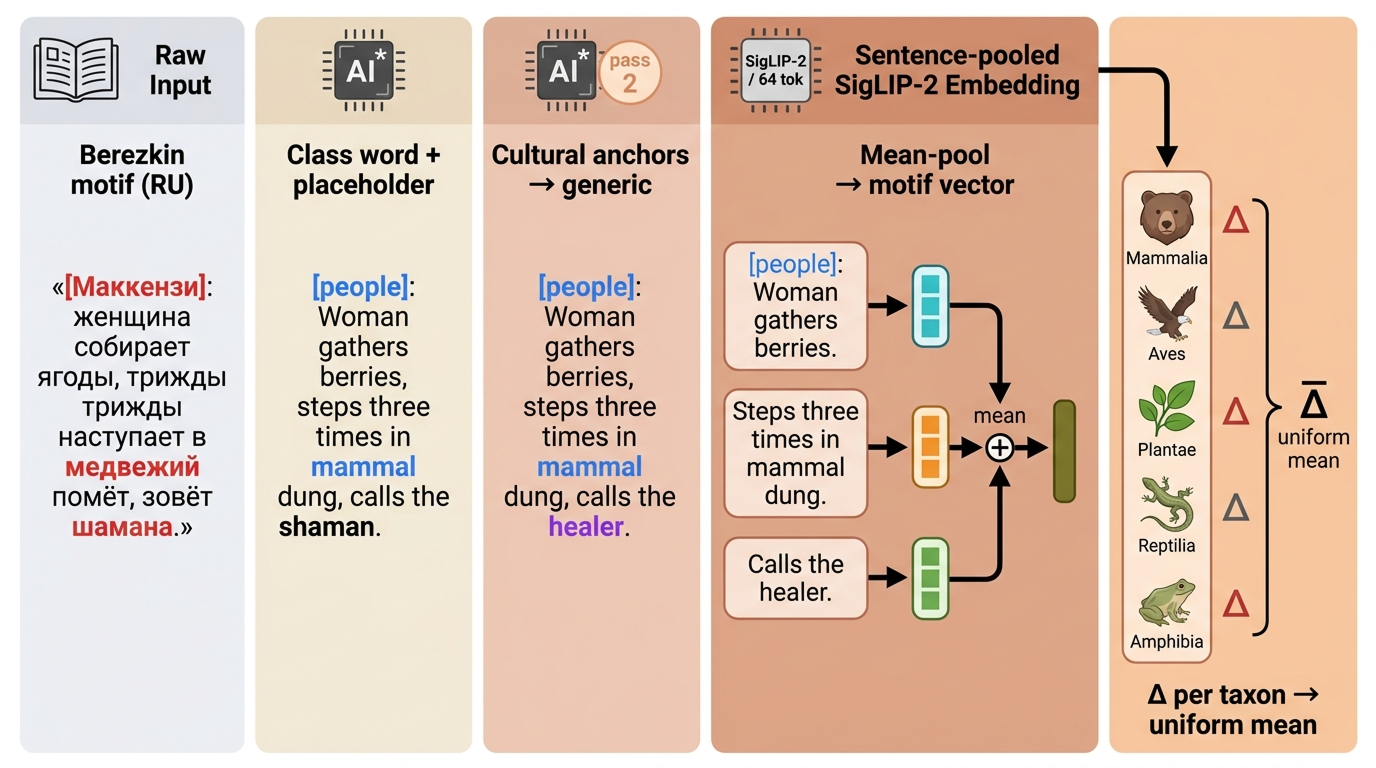
\includegraphics[width=\textwidth]{methods.png}
\caption{\textbf{Pipeline schematic: anonymisation, sentence-
pooled embedding, and image-side stratification.} An example
Berezkin motif (Mackenzie-region tradition, Boreal/Taiga) is
threaded through the five stages of the analysis pipeline so the
reader can trace one token's journey from raw Russian to the
final per-taxon $\Delta$. \emph{Stage 0 (Raw input).} The
Russian motif from Berezkin's catalogue, with biome-anchoring
tokens highlighted in red (the species name ``медвежий'' bear,
the cultural anchor ``шамана'' shaman, the ethnonym
``Маккензи''). \emph{Stage 1 (Class word + placeholder).} An
LLM pass translates the text into English and applies seven
noun-targeted anonymisation rules; specific species names become
their class word (bear $\to$ \texttt{mammal}), ethnonyms become
\texttt{[people]}, biome words are dropped. Replaced tokens are
shown in blue. \emph{Stage 2 (Cultural anchors $\to$ generic).}
A second LLM pass refines long-tail cultural anchors that
survived Stage 1 (\texttt{shaman} $\to$ \texttt{healer},
shown in purple); held-out audit on $200$ random motifs confirms
$96.5\%$ strict-clean rate against species, place, and biome
vocabulary. \emph{Stage 3 (Sentence-pooled SigLIP-2 embedding).}
The cleaned abstract is split into sentences, each sentence is
embedded independently within SigLIP-2's $64$-token window
(mean $23$ sentences per motif; $50{,}032$ total across $2{,}158$
motifs), and the per-motif vector is the mean-pooled,
L2-renormalised sentence embedding. \emph{Stage 4 ($\Delta$ per
taxon $\to$ uniform mean).} On the image side, iNaturalist
photographs of biome $b$ are partitioned by iconic taxon
(Mammalia, Aves, Plantae, Reptilia, Amphibia, \ldots). The
motif vector's residualised $\Delta$ is computed within each
taxon stratum and averaged uniformly across taxa, removing
biome-by-taxon co-occurrence on the image side as a possible
explanation of alignment.}
\label{fig:methods-controls}
\end{figure}

The motif text fed to the encoder is anonymised against every
category of biome-anchoring vocabulary we could identify, by an
LLM-mediated translation and refinement pass followed by a single
exclusion filter. For each motif we send the raw Russian Berezkin
abstract together with the original English oneliner to
gemini-3.5-flash (Google's frontier flash model, released May
2026)~\citep{googlegemini2026} with a structured prompt that asks
it to produce a faithful English translation under the following
rules:

\begin{itemize}\itemsep1pt\parsep0pt
\item Every specific species name $\to$ its class word: one of
  \texttt{mammal} / \texttt{bird} / \texttt{fish} / \texttt{reptile}
  / \texttt{amphibian} / \texttt{insect} / \texttt{mollusc} /
  \texttt{crustacean} / \texttt{arachnid} / \texttt{tree} /
  \texttt{flower} / \texttt{plant} / \texttt{fungus} /
  \texttt{animal}.
\item Every country, region, river, mountain, lake, sea, ocean, or
  city name $\to$ the literal string \texttt{[place]}.
\item Every tribe, ethnic group, nation, or ethno-religious
  community name $\to$ \texttt{[people]}.
\item Every biome word (tundra, taiga, savanna, jungle, rainforest,
  prairie, desert, steppe, swamp, marsh, oasis, glacier, veldt,
  mangrove, mediterranean, etc.) dropped.
\item Every cultivated crop (rice, corn, beans, peanuts, millet,
  quinoa, cassava, cotton, indigo, tobacco, etc.) $\to$
  \texttt{plant}.
\item Every biome-coded cultural artefact (sledge, kayak, harpoon,
  igloo, yurt, blowgun, snowshoes, kachina, calabash) $\to$ a
  generic equivalent (tool, boat, shelter, vessel).
\item Latin binomials dropped.
\end{itemize}

A second Gemini pass applied to the first-pass output catches the
long tail and additionally:

\begin{itemize}\itemsep1pt\parsep0pt
\item Cultural-religious titles (sultan / padishah / shah / kadi /
  mullah / dervish / brahmin / bai / lama / raja / khan / tsar)
  $\to$ neutral ``ruler'' or ``holy person'' or ``wealthy person''
 , explicitly \emph{not} the Western-coded ``king'' / ``queen''
  / ``priest'' / ``monk''.
\item Tradition-specific named characters (Baba~Yaga, Kivioq,
  Coyote-as-character, Nach Ak Yum, Quetzalcoatl, Khevki,
  Mitoshka, etc.) $\to$ ``character''.
\end{itemize}

Kept by design as cross-cultural anchors: cross-cultural religious
figures (Christ, Buddha, Adam, Eve, Allah, God, Satan, named
saints, Krishna, Rama, Sita), universal personifications (Sun,
Moon, Wind, Sky, Earth, Sea, Thunder, Lightning, Star), all
astronomical references (Pleiades, Orion, Big Dipper, Sirius,
Venus, Milky Way, named constellations), all class words, cardinal
directions, and generic universal vocabulary (forest, mountain,
river, village, house, person, woman, man, child, day, night,
fire, water). The narrative content of each motif, transformations,
family relationships, magical events, plot, is preserved.

A held-out audit of $200$ random LLM-anonymised motifs (criteria
itemised in the Results panel C) finds $0\%$ explicit biome
words, $0.5\%$ place or ethnonym residues, and $3.0\%$ specific
species residues, giving a composite strict-clean rate of
$96.5\%$ against species, place, and biome vocabulary. Generic
landform vocabulary (forest, mountain, river, snow, sand,
$92.5\%$ of motifs) and biome-correlated activity verbs (gather,
hunt, fish, herd, $93.5\%$ of motifs) are retained by
construction: the anonymisation pipeline is \emph{noun-targeted},
stripping species, place, biome, and cultural-artefact nouns
while leaving narrative structure and activity predicates intact.
A residual narrative such as ``gathers fruit, steps in mammal
dung'' therefore retains activity-level biome correlates
(gathering fruit is more frequent in temperate and boreal forest
descriptions than in desert ones). We treat this retained
content as the substrate over which the alignment is measured
rather than as contamination, and return to the
morphology-versus-activity-priming question in the Discussion.

\subsubsection*{Within-taxon image-side stratification.}
Because iNaturalist observations are taxonomically structured, some
biomes are disproportionately rich in particular iconic taxa
(boreal/tundra/conifer forests are $55$--$66\%$ Plantae; mangroves
only $11\%$). A motif whose anonymised text emphasises one taxon
class will therefore score high in any biome whose iNat image pool
emphasises the same taxon class, even when the biome's specific
visual character contributes nothing. To remove this biome-by-taxon
co-occurrence as a possible explanation for the alignment, we
recompute $\Delta_b$ stratified by the iNaturalist iconic-taxon
label. For each biome $b$ and taxon stratum $t$ with at least $20$
images, we compute the within-stratum
$\Delta_{b,t} = \overline{S_{i,\mathcal{M}_b}}_{i\in b\cap t}
              - \overline{S_{i,\mathcal{M}_{\overline{b}}}}_{i\in b\cap t}$,
and report the uniform across-strata mean as
$\Delta^{\text{strat}}_b = (1/T_b)\sum_t \Delta_{b,t}$. The
permutation null is the same scrambled-motif null applied within
strata. The headline iNaturalist statistic reported throughout the
main text and main figures is stratified
($\mu\Delta^{\text{strat}} = +0.406\times 10^{-3}$ across the 14
biomes), with the marginal $\mu\Delta^{\text{marg}} = +0.244\times
10^{-3}$ reported alongside in robustness panels (where the
input rather than the statistic is being varied) and on the
Places365 panel of Figure~\ref{fig:fig2} (Places365 has no
iconic-taxon labels and therefore admits no further
stratification). Per-text-taxon decompositions
(Figure~\ref{fig:fig10}) report the per-cell marginal value at
each biome--taxon cell, since each cell already conditions on a
single taxon; the stratified $\Delta$ is, mechanically, the
uniform mean of those per-cell marginals.

We separately explored simpler rule-based anonymisation pipelines
(genus-level hypernymisation; a hand-curated class-level Russian
hypernym map of roughly $3{,}500$ entries; an audit-extended map
of $6{,}300$ entries) and found that the effect is positive under
each of them and the across-biome ranking is preserved, ruling out
the interpretation that any particular vocabulary anchor is doing
the work. The LLM-mediated pipeline described above is the
strictest in the family and the one we use for the headline.

\subsection*{Identity-naming controls}

To test the alignment on the un-anonymised myths while controlling
for biome-correlated naming, we extracted three identity classes
per motif from the raw Russian Berezkin abstracts and kept them
separate. Species (every specifically named organism, fauna and
flora) were extracted by an LLM reading the Russian text; a
held-out adversarial audit of $120$ motifs estimated $96.7\%$
recall and $95.3\%$ precision against the source. Places are the
WWF-codable regions in Berezkin's metadata, and ethnonyms are the
tradition names that carry each motif. Each class was rendered as a
bag of its entities, embedded with the same sentence-pooled
SigLIP-2 pipeline as the full myth in the raw-Russian frame, and
scored against the same iNaturalist images on the within-iconic-
taxon stratified $\Delta$. Because this is a self-contained
raw-Russian decomposition, its absolute magnitudes are not
formally comparable to the English LLM-clean headline, although the
full-myth stratified $\Delta$ coincides closely with it. The
matched-permutation null partitions motifs into $60$ K-means blocks
in the relevant identity-bag embedding space and, for each of
$1{,}000$ permutations, shuffles biome labels only within a block,
so identity content is held approximately constant while biome
assignment is broken; the joint null concatenates the
L2-normalised species, place, and ethnonym embeddings before
blocking. Each biome is tested with an independent random-number
stream, permutation $p$-values are $(1+\#\{null \geq obs\})/(1+1000)$
smoothed, and significance is reported after Benjamini--Hochberg FDR
correction across the 14 biomes; the survivor counts in
Figure~\ref{fig:fig-identity}B are at $q<.05$. The species-subspace
projection removes the top $k$ principal directions of the
species-bag embeddings from the full-myth embeddings
($k = 5, 10, 20$) and recomputes the stratified $\Delta$. The
extraction prompts, audit, and per-biome tables are released with
the code.

\subsection*{Statistical tests}

Image--motif similarities form an
$n_{\text{img}} \times n_{\text{motif}}$ matrix~$\mathbf{S}$.
Per-motif residualisation (subtracting the motif grand mean)
eliminates the contribution of generic motif valence to per-biome
aggregates. For each biome $b$ with $n_b$ images and motif
partition $(\mathcal{M}_b, \mathcal{M}_{\overline{b}})$ where
$\mathcal{M}_b$ is the set of motifs whose Berezkin tradition set
includes at least one tradition assigned to biome $b$, we report
\[
\Delta_b \;=\; \frac{1}{n_b}\sum_{i \in \text{imgs}(b)}
        \Bigl[\,\overline{S_{i,\mathcal{M}_b}}
            - \overline{S_{i,\mathcal{M}_{\overline{b}}}}\,\Bigr],
\]
the residualised marginal $\Delta$ at the biome level. The
headline iNat statistic is the within-iconic-taxon stratified
version $\Delta^{\text{strat}}_b$ defined above. Significance is
assessed by $1{,}000$ permutations of the motif-to-biome
assignment (with the stratified statistic recomputed under each
permutation), with FDR control across biomes via the
Benjamini--Hochberg procedure~\citep{benjamini1995controlling}.
For all main-figure panels we apply a display threshold of
$\geq 50$ in-biome images, $\geq 5$ in-biome motifs, and
$\geq 20$ images per biome--taxon stratum; biome--taxon cells
with fewer than $10$ images appear as missing in the per-taxon
decomposition (Figure~\ref{fig:fig10}).

\subsection*{Unsupervised biome recovery}

To test whether biome structure is present in the model's image
affinities without supervision, we represented each of the
$2{,}158$ valid motifs by its row of the residualised similarity
matrix $\mathbf{S}$, that is, its per-motif-centred cosine
similarity to all $46{,}481$ iNaturalist photographs, and reduced
these affinity vectors to $50$ principal components. A motif's
\emph{own biome} is the biome contributing the most of its Berezkin
traditions; this label is used only to evaluate the geometry, never
to build it. We report two diagnostics over the nine biomes with
at least $50$ images and $20$ own-biome motifs. First, own-biome
retrieval: for each motif we computed a taxon-stratified mean
similarity to each biome (the mean over iconic taxa of the motif's
mean similarity to that biome's images of each taxon, requiring
$\geq 20$ images per biome--taxon cell), ranked the biomes, and
recorded the rank of the motif's own biome; the chance baseline and
the reported $p$-value come from $2{,}000$ permutations that
reassign each motif's own biome at random. Second, per-biome
decodability is the balanced accuracy of a five-fold
one-versus-rest $\ell_2$-regularised logistic probe on the
PCA-reduced vectors, compared against a null of $200$ such probes
trained on permuted labels (each biome with an independent stream),
with per-biome $p$-values smoothed as
$(1+\#\{null\geq obs\})/(1+200)$ and Benjamini--Hochberg FDR
correction across the nine biomes. The unsupervised UMAP layout and its
content, macro-area, and biome adjusted Rand indices use the same
PCA-reduced vectors. As a text-side control against the taxon
channel, both diagnostics are recomputed on the class-word-collapsed
embeddings (every animal-kingdom class word mapped to ``animal'' and
every plant-kingdom class word to ``plant''; see \emph{Controls
against biome cues}).

% =============================================================================
\section*{Data and code availability}
All code, sentence-pooled SigLIP-2 embeddings, the LLM-clean motif
texts (Gemini-3.5-Flash output), the held-out anonymisation audit
(the per-criterion coding of the 200 audited motifs is released as
\texttt{anonymisation\_audit\_200motif.csv}), and the earlier
rule-based hypernym maps released for completeness are available at
[repository URL placeholder]. The Berezkin
abstracts are accessible at
\url{http://www.ruthenia.ru/folklore/berezkin/}.

\section*{Acknowledgements}
[Placeholders.]

% =============================================================================
\bibliography{references}

% =============================================================================
\appendix
\section*{Supplementary materials}\label{app:supp}

The supplementary materials below collect the analyses that probe
the robustness of the headline finding from five complementary
angles: (i) the headline robustness atlas (word-shuffle, encyclopedic-
register null, and baseline controls), with the four panels shown at
full size; (ii) a
per-taxon decomposition that asks which iNaturalist taxonomic
groups carry the alignment; (iii) a cross-model replication
across four vision--language model architectures on the same
LLM-clean text; (iv) two analyses directly addressing whether
biome-correlated lexical content in the cleaned text could by
itself explain the alignment (a high-tell versus low-tell split
and a within-Glottolog-macroarea biome-swap null); and (v) an
analysis of the raw ecological composition of motif text per
biome, which makes explicit what the anonymisation pipeline is
removing. Throughout, the same statistical conventions apply as
in the main text: sentence-pooled SigLIP-2 on the full LLM-clean
corpus, residualised $\Delta$ with $1{,}000$ motif-to-biome
permutations and Benjamini--Hochberg FDR within each panel, and
gold marks for $q < 0.05$.

\subsection*{S1. Robustness atlas}

Four robustness analyses bound where the headline signal comes
from. Word-shuffling each motif before sentence-pooling leaves
the stratified $\mu\Delta$ essentially unchanged, indicating that
the alignment depends on lexical content rather than narrative
structure. Replacing the motifs with synthetic
encyclopedic-register paragraphs of comparable length collapses
$\mu\Delta$ to near zero, ruling out the possibility that the
residualised statistic produces a positive bias on biome-neutral
text. The per-biome $\Delta$ also replicates across all four
vision--language model architectures we tested (SigLIP-2 sentence-
pooled, M-CLIP, OpenCLIP-LAION-2B, OpenCLIP-OpenAI) with
across-model Pearson correlations between $+0.74$ and $+0.94$,
ruling out a SigLIP-specific training-distribution artefact.
Finally, a held-out audit of 200 random anonymised motifs
confirms a strict-clean rate of $96.5\%$ against species, place,
and biome vocabulary; the categories that remain by construction
(generic landform words, activity verbs) are the substrate over
which we measure alignment, and we interpret them as such in the
main text Discussion.

\begin{figure}[h!tbp]
\centering
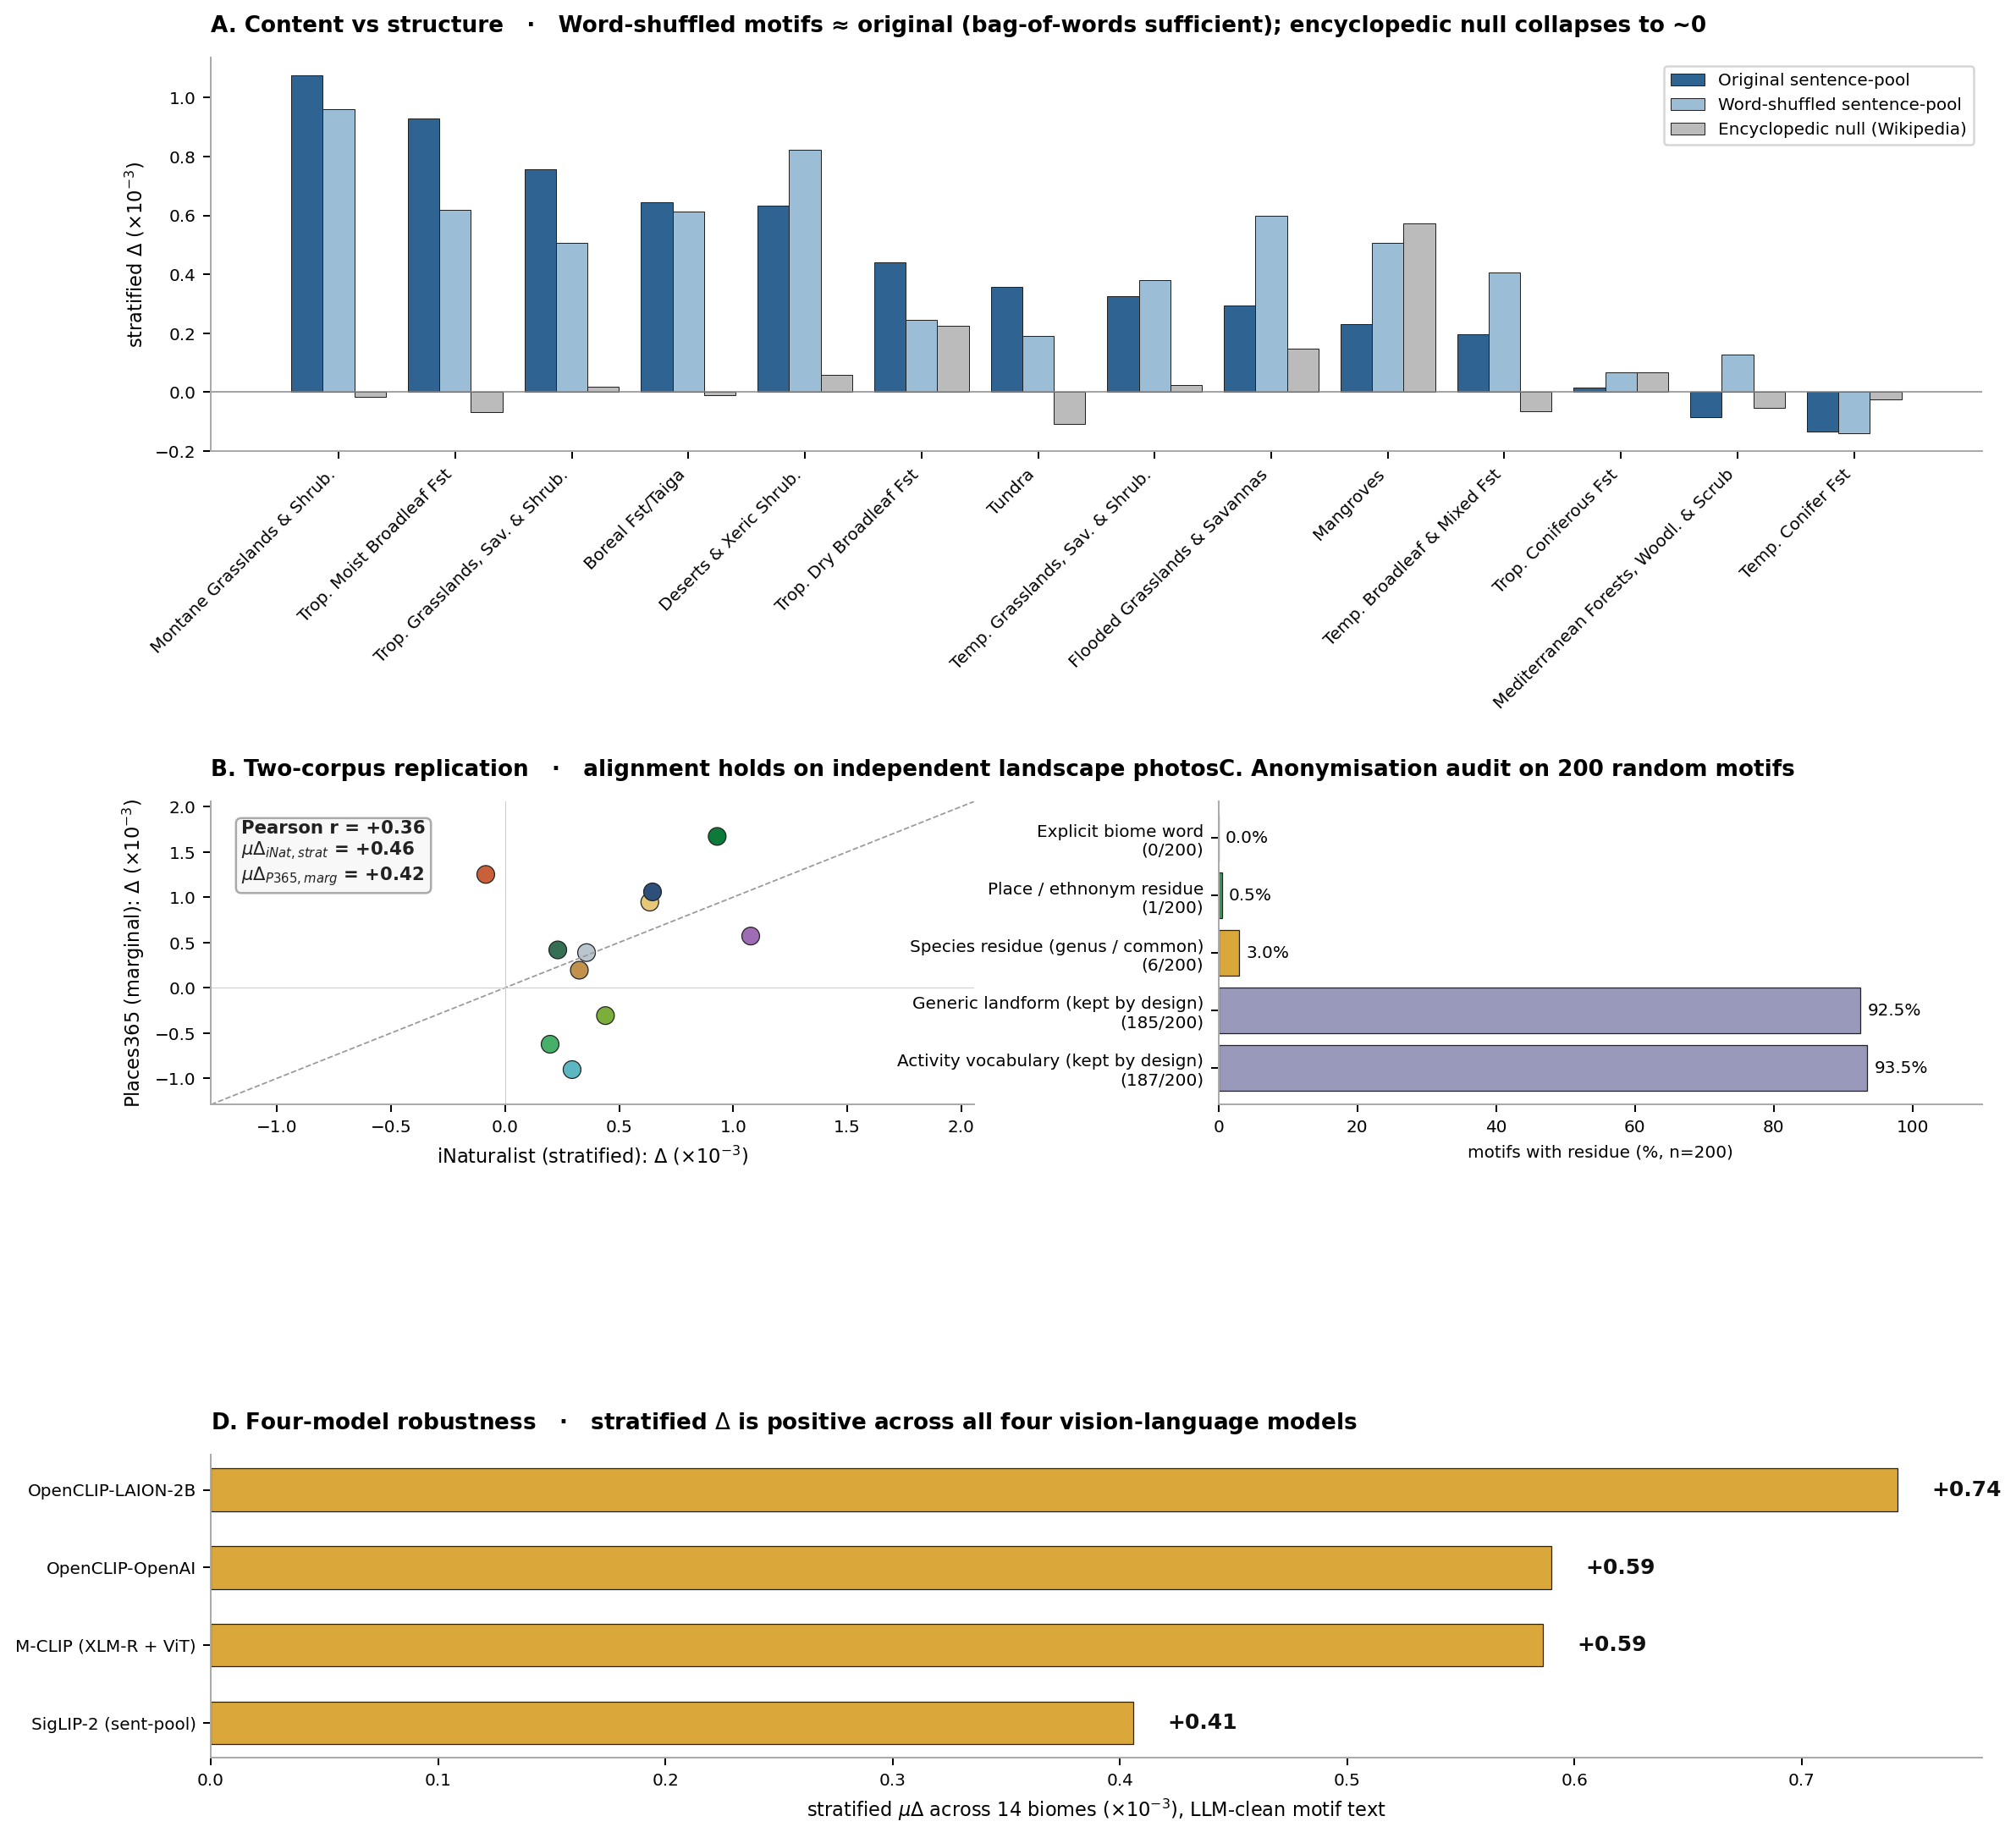
\includegraphics[width=\textwidth]{fig_v2_controls.png}
\caption{\textbf{Robustness atlas referenced in the main
Results.} \emph{Panel A}: per-biome stratified $\Delta$ on
iNaturalist under three conditions that modify the text input.
The original sentence-pooled embedding (dark blue) is essentially
identical to its word-shuffled version (light blue) at every
biome, indicating that the alignment depends on lexical content
rather than narrative structure. The encyclopedic null (grey),
in which synthetic encyclopedic-register English paragraphs of
comparable length replace the LLM-clean motifs, collapses the
alignment toward zero across biomes.
\emph{Panel B}: per-biome stratified $\Delta$ on iNaturalist
species photographs (x-axis) versus marginal $\Delta$ on
Places365 landscape scenes (y-axis), one point per WWF biome that
both corpora cover. Pearson $r = +0.36$ across the 11 shared
biomes; mean $\Delta$ positive on both sides ($+0.46\times
10^{-3}$ iNat-shared stratified, $+0.42\times 10^{-3}$ Places365
marginal). The two corpora share no images and no visual content
type, so this is an independent cross-channel replication.
\emph{Panel C}: expanded $200$-motif audit, per-criterion
residue rate. Biome words, place or ethnonym residues, and
specific species references are essentially eliminated ($0\%$,
$0.5\%$, and $3.0\%$ respectively; composite strict-clean rate
$96.5\%$). Generic landform vocabulary and biome-correlated
activity verbs are retained by design.
\emph{Panel D}: cross-model headline stratified $\mu\Delta$ on
the same LLM-clean motif text. Stratified $\mu\Delta$ is positive
on all four architectures, from $+0.41\times 10^{-3}$ on
SigLIP-2 to $+0.74\times 10^{-3}$ on OpenCLIP-LAION-2B.}
\label{fig:v2controls}
\end{figure}

\subsection*{S2. Per-taxon decomposition (small-multiples view)}

Figure~\ref{fig:figS-taxonfacets} re-renders the per-taxon
decomposition of the headline result as small-multiple bar panels,
one taxon per panel, with within-taxon BH-FDR. This is a
complementary view of the same data as Figure~\ref{fig:fig10}: rather
than collapsing a taxon's twelve biome cells into one violin, each
panel shows the per-biome $\Delta$ values themselves, so the reader
can see which specific biomes carry each taxon's effect. The
``all'' panel reproduces the headline ranking (Tropical Grasslands,
Mediterranean, Boreal/Taiga at the top); the Aves and Plantae panels
echo this pattern; the Reptilia, Mollusca, and Arachnida panels show
little structure, consistent with the per-taxon violin summary.

\begin{figure}[h!t]
\centering
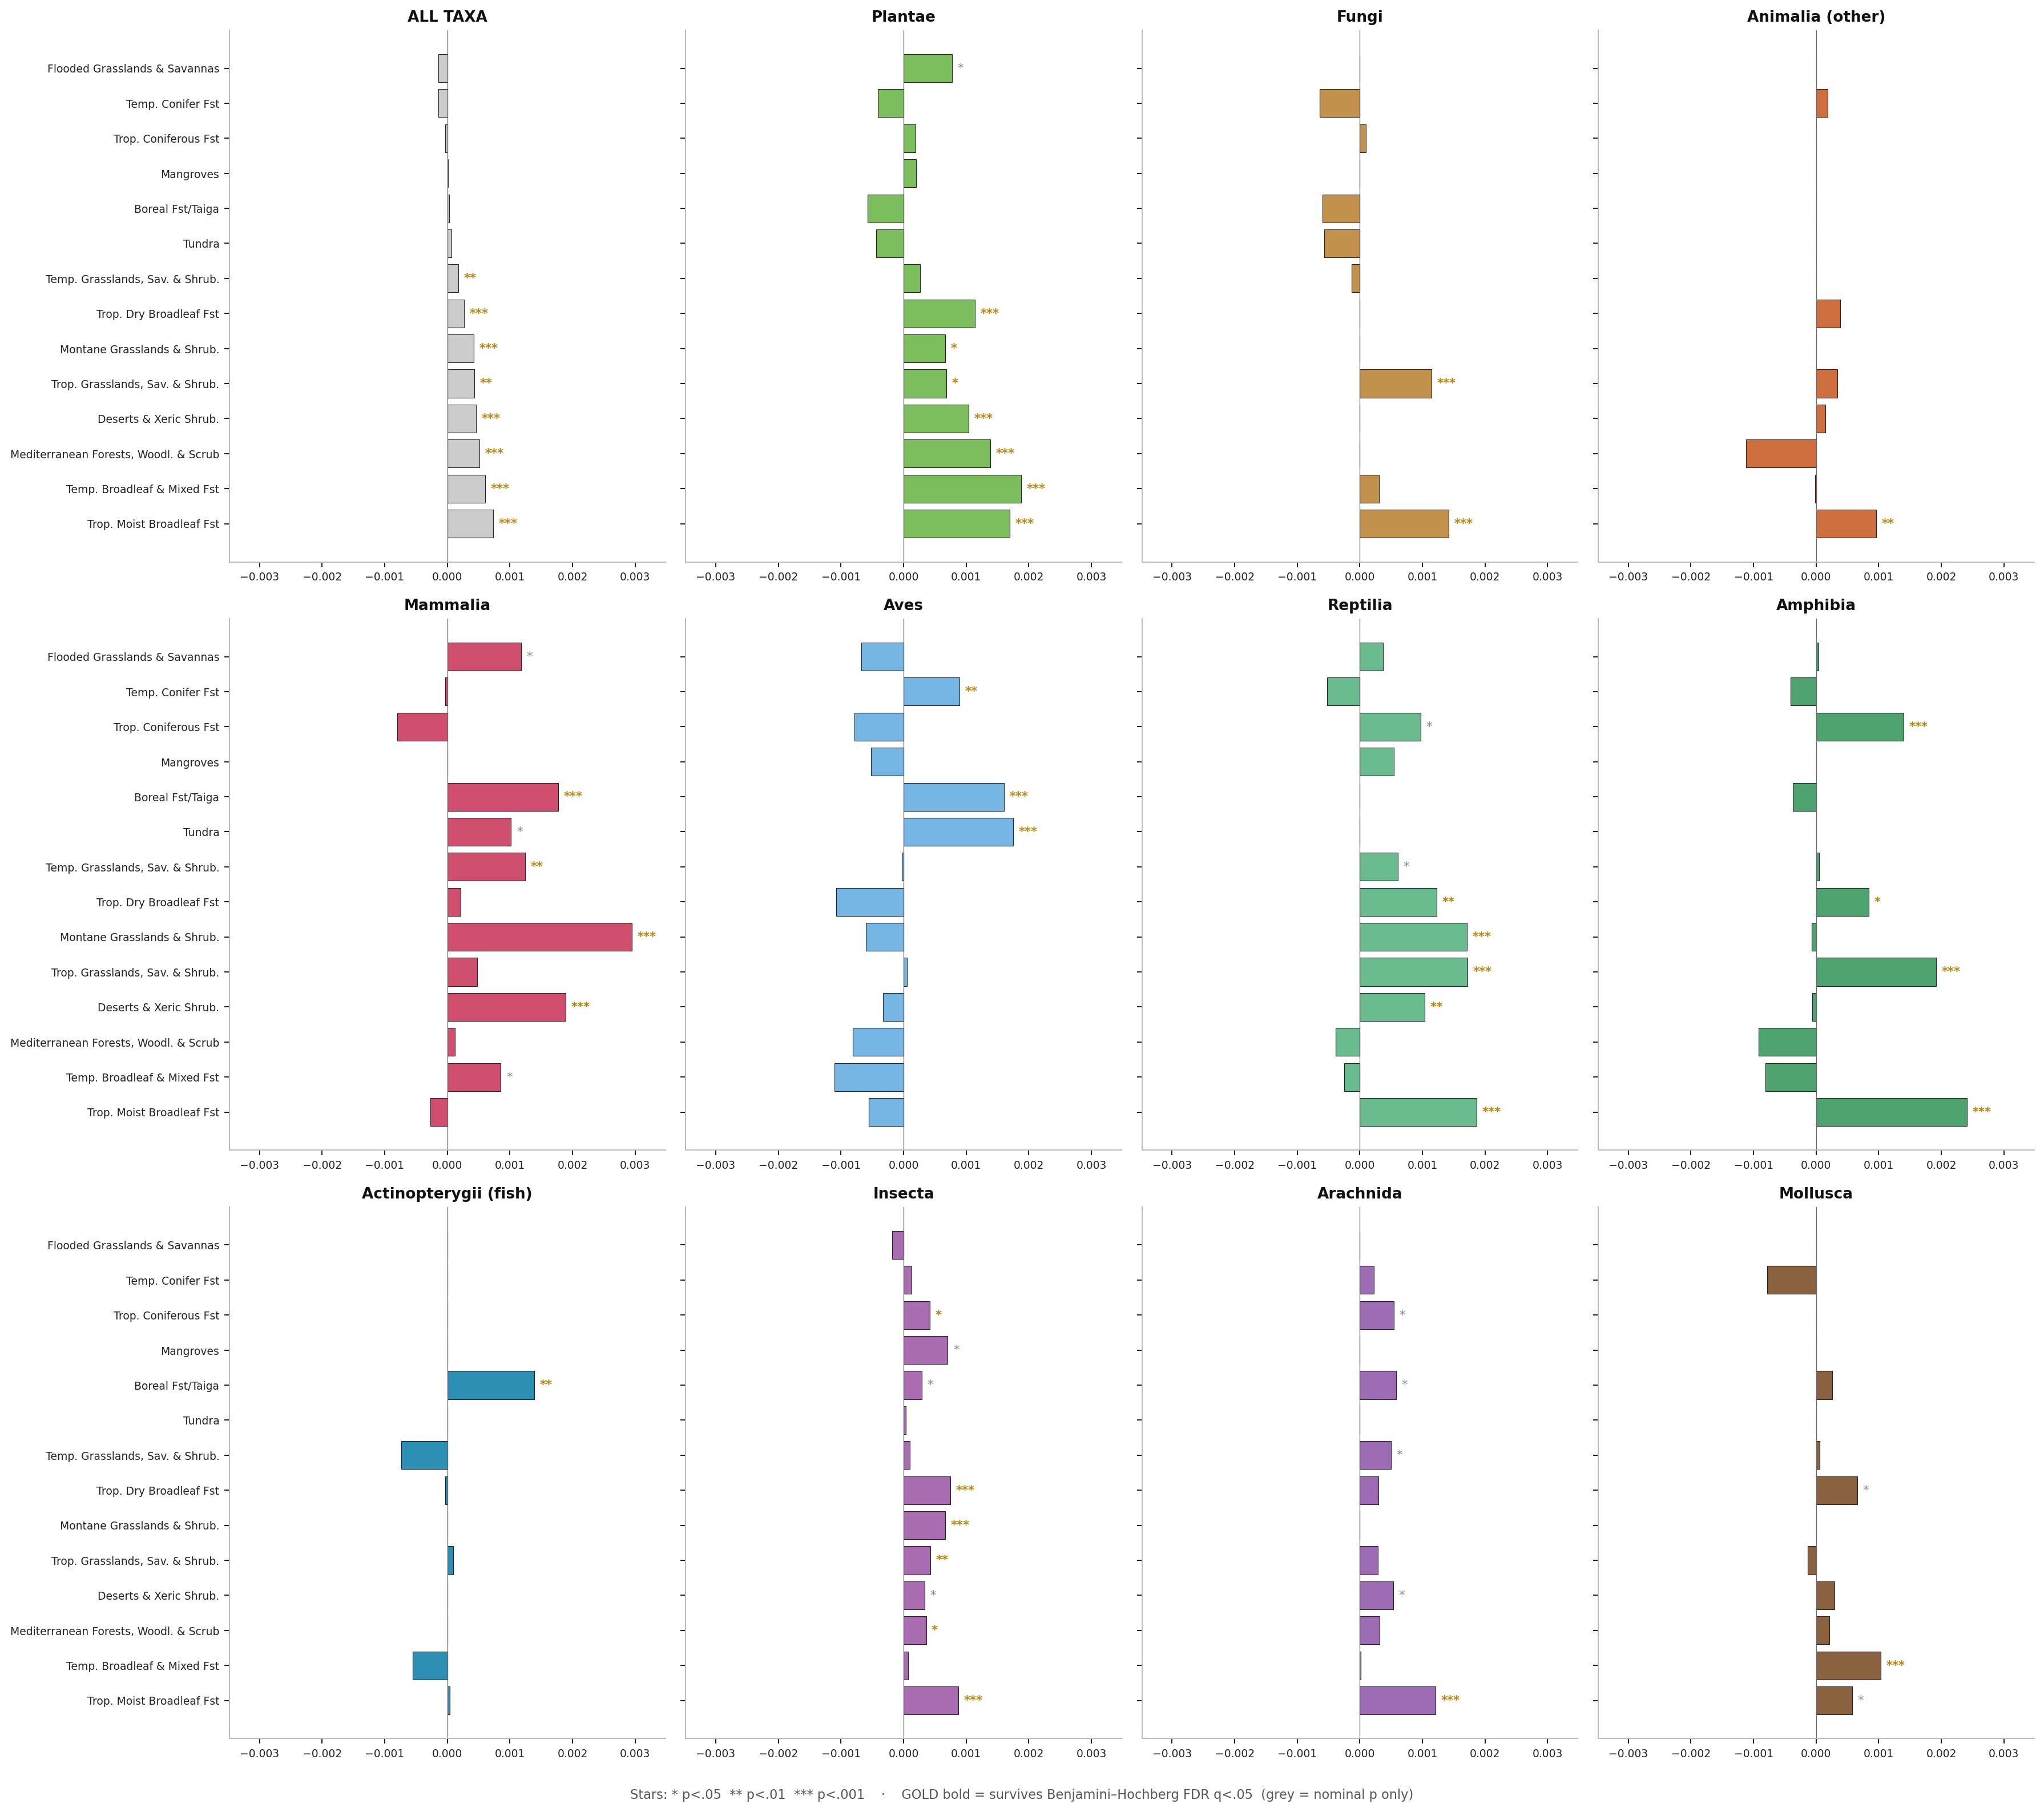
\includegraphics[width=0.95\textwidth]{fig4_taxon_facets.png}
\caption{\textbf{Per-taxon biome panels.} Per-taxon decomposition of
the headline result, presented as small-multiple bar panels with
within-taxon BH-FDR. Each panel shows the per-biome $\Delta$ for one
taxon; biome row order is preserved across panels. Gold stars mark
BH-$q < 0.05$ within the panel. Complements
Figure~\ref{fig:fig10}.}
\label{fig:figS-taxonfacets}
\end{figure}

% S2. Anonymisation-progression robustness ladders removed
% (Fig 8 + Fig 9 in earlier numbering). The naming-progression ladders
% compared the LLM-mediated headline pipeline against earlier
% rule-based hypernym maps (v3 / v4 / v6 / v7 / v8). The progression
% was useful as evidence that the effect is not specific to one
% anonymisation choice, but presenting it alongside the LLM headline
% invites the reader to weigh methods that were subsequently
% superseded. The robustness claim is preserved verbally in the
% Methods section.

\subsection*{S3. Cross-model replication}

Figure~\ref{fig:figS-crossmodel} tests whether the per-biome
stratified $\Delta$ pattern is an artefact of the specific
vision--language model architecture used to produce the
embeddings (sentence-pooled SigLIP-2-large in the headline
analysis). For this robustness check we re-run the within-iconic-
taxon stratified pipeline with four distinct vision--language
model families on the same LLM-clean English motif text:
sentence-pooled SigLIP-2-large; M-CLIP (XLM-Roberta-Large paired
with CLIP-ViT-L/14, $512$-token native window);
OpenCLIP-ViT-L/14-LAION-2B; and OpenCLIP-ViT-L/14-OpenAI. The
$4 \times 4$ scatter matrix shows per-biome stratified $\Delta$
correlations for every model pair; the off-diagonal cells report
Pearson $r$. Correlations lie in $[+0.74, +0.94]$ across all six
distinct model pairs, with the SigLIP-2-vs-OpenCLIP-LAION-2B
pair carrying the strongest agreement ($r = +0.94$). The
per-biome ranking is preserved across every model family tested,
ruling out reading on which the headline pattern is a
SigLIP-2-specific artefact of one model's training distribution.

\begin{figure}[h!t]
\centering
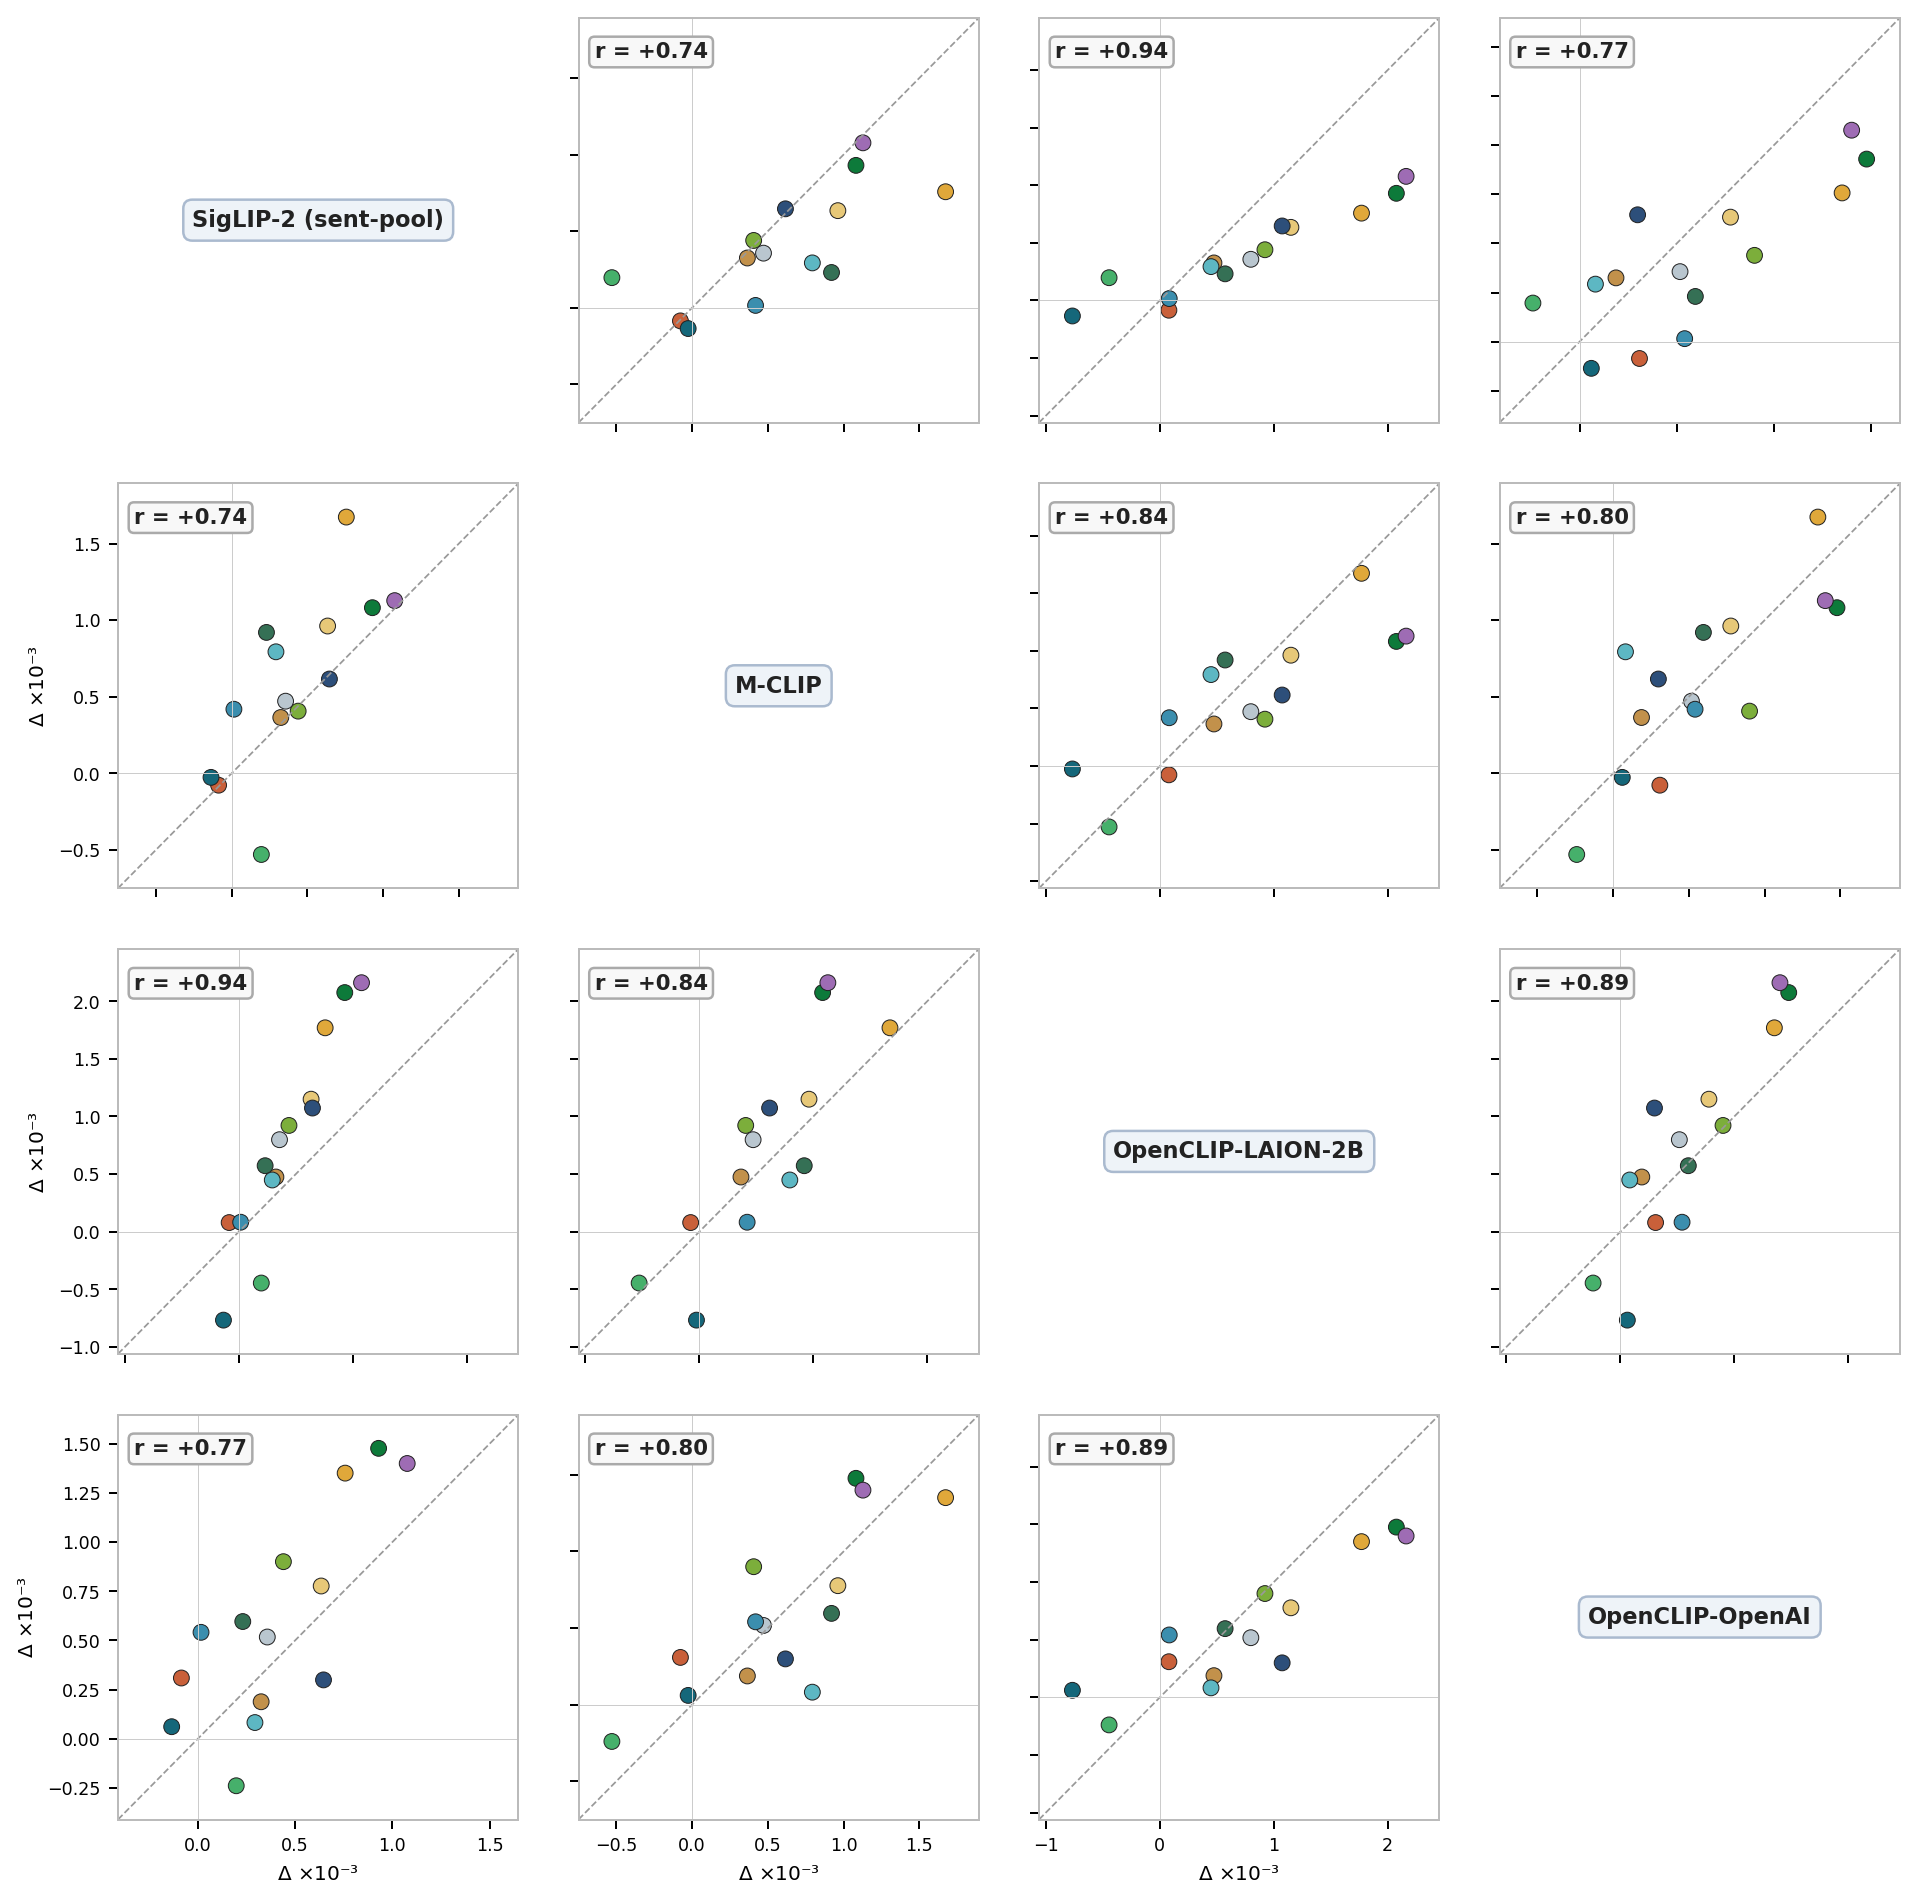
\includegraphics[width=\textwidth]{fig9_crossmodel_correlation.png}
\caption{\textbf{Cross-model robustness.} $4 \times 4$ scatter
matrix of per-biome within-iconic-taxon stratified $\Delta$ on
the same LLM-clean Berezkin abstracts and the same iNaturalist
images, across four vision--language model architectures.
Off-diagonal cells report Pearson $r$ between models; the dashed
line marks $y = x$. Each point is one of the 14 WWF biomes,
coloured by the standard biome palette. All six distinct model
pairs correlate in $[+0.74, +0.94]$.}
\label{fig:figS-crossmodel}
\end{figure}

\subsection*{S4. Biome-tell tests}\label{sec:biome-tell}

A residual concern about the headline alignment is that the
anonymised text might still contain enough biome-correlated
vocabulary (generic landform words, activity verbs,
class-level animal terms) for SigLIP-2 to recover biome
assignment from text alone, with the image side being a
secondary recovery of that lexical signal rather than an
independent confirmation. We address this concern with two
analyses whose details are provided in the data drop.

\paragraph*{High-tell versus low-tell split.} For each motif we
compute a biome-tell $z$-score: the gap between its maximum
sentence-pooled SigLIP-2 similarity to its assigned biomes'
visual prototypes and the mean similarity to non-assigned
biomes' prototypes, normalised by the standard deviation of
off-target similarities. We split motifs at the median tell
$z$-score and run the within-iconic-taxon stratified $\Delta$
test on each half (Table~\ref{tab:biome-tell-split}). The
high-tell half (motifs whose anonymised text \emph{is} biome-
recoverable above chance) gives $\mu\Delta^{\text{strat}} =
+0.54\times 10^{-3}$ with 7 of 14 biomes significant at $p<.05$;
the low-tell half (motifs whose anonymised text alone is
\emph{least} biome-recoverable) still gives $\mu\Delta^{
\text{strat}} = +0.21\times 10^{-3}$ with 7 of 14 biomes
significant at $p<.05$. Text-only biome predictability therefore
contributes to the alignment (the high-tell half is about $2.5
\times$ the low-tell half), but the low-tell half on its own is
not zero. That motifs whose text alone provides minimal biome
predictability still align positively with their biome's
imagery indicates that the headline signal is not fully
explained by biome-correlated lexical content recoverable from
text alone.

\begin{table}[h!]
\centering
\caption{High-tell versus low-tell split. Median-split of motifs
on the biome-tell $z$-score (text-only biome predictability),
with the within-iconic-taxon stratified $\Delta$ test recomputed
on each half on iNaturalist images. Both halves carry a positive
across-biome mean $\Delta$.}\label{tab:biome-tell-split}
\begin{tabular}{lrrr}
\hline
Subset & $\mu\Delta^{\text{strat}}$ ($\times 10^{-3}$) & $\mu\Delta^{\text{marg}}$ ($\times 10^{-3}$) & Sig $p<.05$ \\
\hline
Low-tell half  & $+0.21$ & $-0.41$ & 7/14 \\
High-tell half & $+0.54$ & $+0.78$ & 7/14 \\
\hline
\end{tabular}
\end{table}

\paragraph*{Within-Glottolog-macroarea biome-swap null.} A
stronger version of the macro-area block-permutation null is to
actively swap biome labels while preserving cultural geography.
For each tradition we randomly reassign its motifs to another
tradition in the same Glottolog macro-area but a \emph{different}
biome, and recompute the per-biome stratified $\Delta$ under each
of $1{,}000$ such swaps. If biome assignment is doing the work,
the swapped Δ should collapse below the observed value; if biome
identity is irrelevant and the alignment is purely a
within-macro-area lexical artefact, the swap distribution should
contain the observed value. Six biomes carry observed stratified
$\Delta$ above the $95$th percentile of the swap null
distribution: Montane Grasslands \& Shrublands (observed $+1.08
\times 10^{-3}$, swap-null mean $+0.09$, $p<.001$), Tropical \&
Subtropical Moist Broadleaf Forests (observed $+0.93$, null mean
$-0.16$, $p<.001$), Boreal Forests/Taiga (observed $+0.65$, null
mean $+0.08$, $p<.001$), Deserts \& Xeric Shrublands ($+0.63$ vs
null $+0.22$, $p=.018$), Tropical \& Subtropical Grasslands \&
Savannas ($+0.76$ vs null $+0.45$, $p=.019$), and Temperate
Grasslands, Savannas \& Shrublands ($+0.33$ vs null $+0.02$,
$p=.022$). The remaining biomes either have observed values
indistinguishable from the swap null (Tundra, Mediterranean,
Temperate Conifer, Temperate Broadleaf) or are too sparsely
represented for a stable swap distribution (Mangroves, Flooded
Grasslands). This is a substantially stronger test than the
standard motif-to-biome permutation, because it preserves
within-macro-area cultural autocorrelation by construction: the
biome label is being shuffled among traditions that share a
linguistic-cultural region. That six biomes still carry signal
above this stricter null indicates the alignment is not fully
explained by within-macro-area lexical regularities --- the
biome content of the motif text itself carries information
beyond what would be recoverable from cultural-region membership
alone.

\begin{figure}[h!t]
\centering
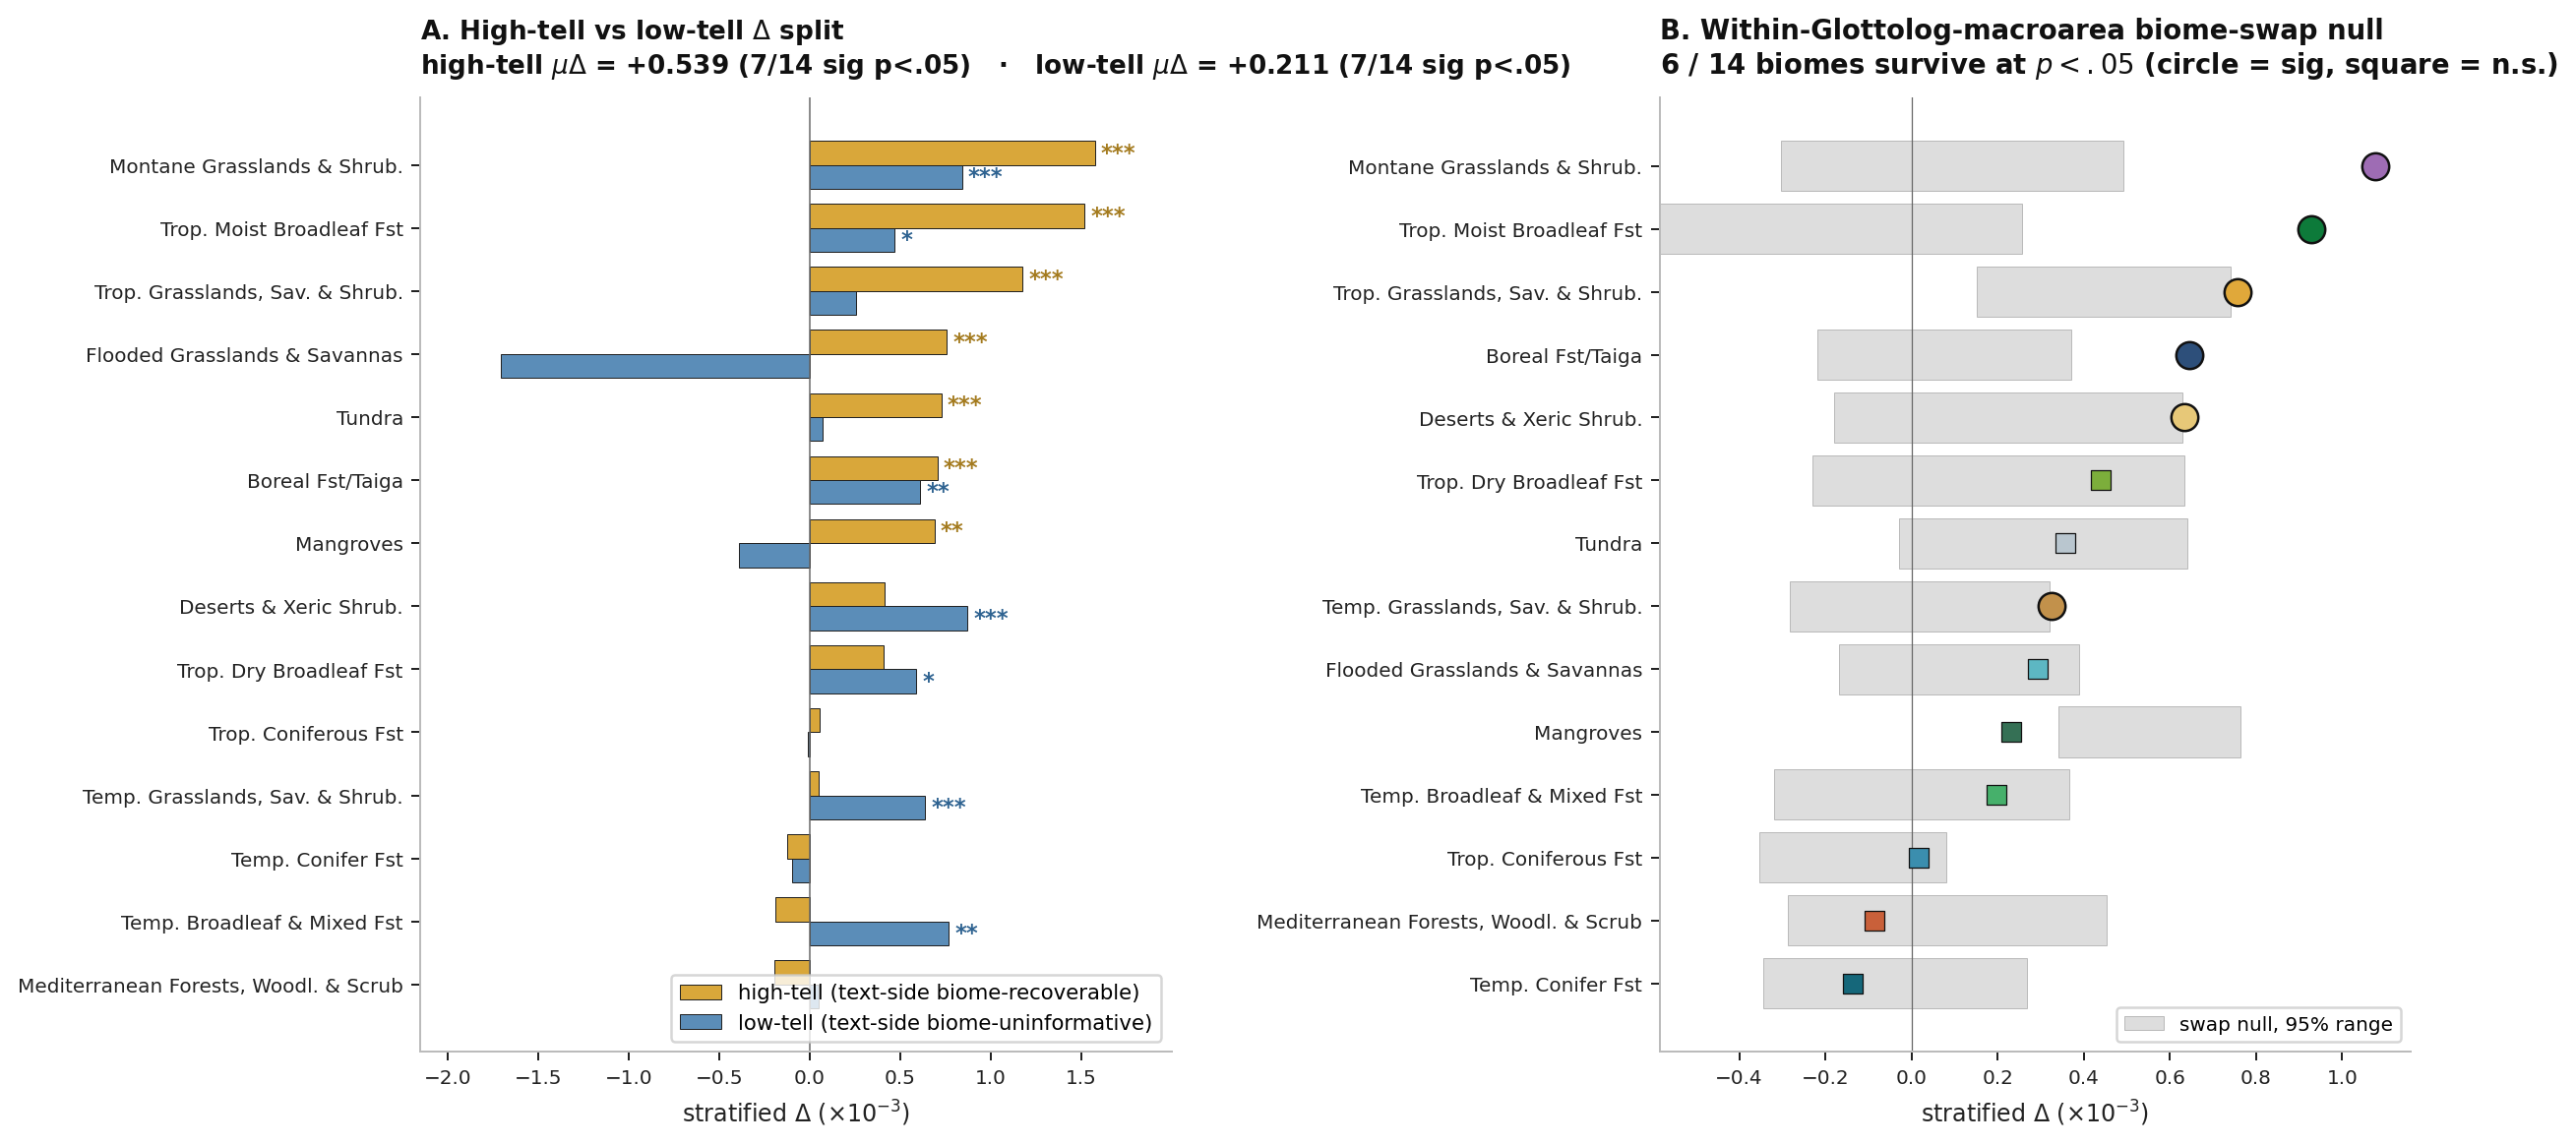
\includegraphics[width=\textwidth]{figS_biome_tell.png}
\caption{\textbf{Biome-tell tests.} \emph{Panel A:} per-biome
within-iconic-taxon stratified $\Delta$ on the high-tell half
(motifs whose anonymised text is biome-recoverable above chance,
gold bars) and the low-tell half (motifs whose text alone is
biome-uninformative, blue bars), across the 14 WWF biomes. Both
halves carry positive across-biome mean $\Delta$ ($+0.54$ and
$+0.21\times 10^{-3}$ respectively); seven biomes are individually
significant at $p<.05$ in each half. \emph{Panel B:} observed
stratified $\Delta$ per biome (coloured markers) overlaid on the
$95\%$ range of the within-Glottolog-macroarea biome-swap null
distribution (grey strips). Circles mark biomes whose observed
$\Delta$ exceeds the $95$th percentile of the swap null
($p<.05$); squares mark biomes that do not. Six biomes survive
this stricter null, indicating that biome content carries
information beyond within-macro-area cultural autocorrelation.}
\label{fig:figS-biome-tell}
\end{figure}

\subsection*{S5. Raw ecological composition per biome (Spec~A view)}

Figure~\ref{fig:figS-species} reports the raw ecological composition
of motif text per biome, before anonymisation. For each WWF biome
(rows) and each of fourteen taxonomic and botanical categories
(columns), the left panel of the heatmap shows the percentage of
Spec~A motifs whose raw Russian abstract mentions at least one
species or plant of that category. The right panel shows the
difference between the Spec~A subset and the all-in-biome pool: a
positive cell means the category is over-represented in
biome-specific motifs relative to the universal-dominated full
pool. The heatmap therefore makes explicit, at the textual level,
which taxonomic categories carry biome-specific signal before the
hypernymisation layer removes their names from the encoder's
input. The figure helps motivate which species-vocabulary
categories the v7 hypernym map needed to cover comprehensively, and
clarifies the ecological content the encoder is no longer
reading at the headline stage.

\begin{figure}[h!t]
\centering
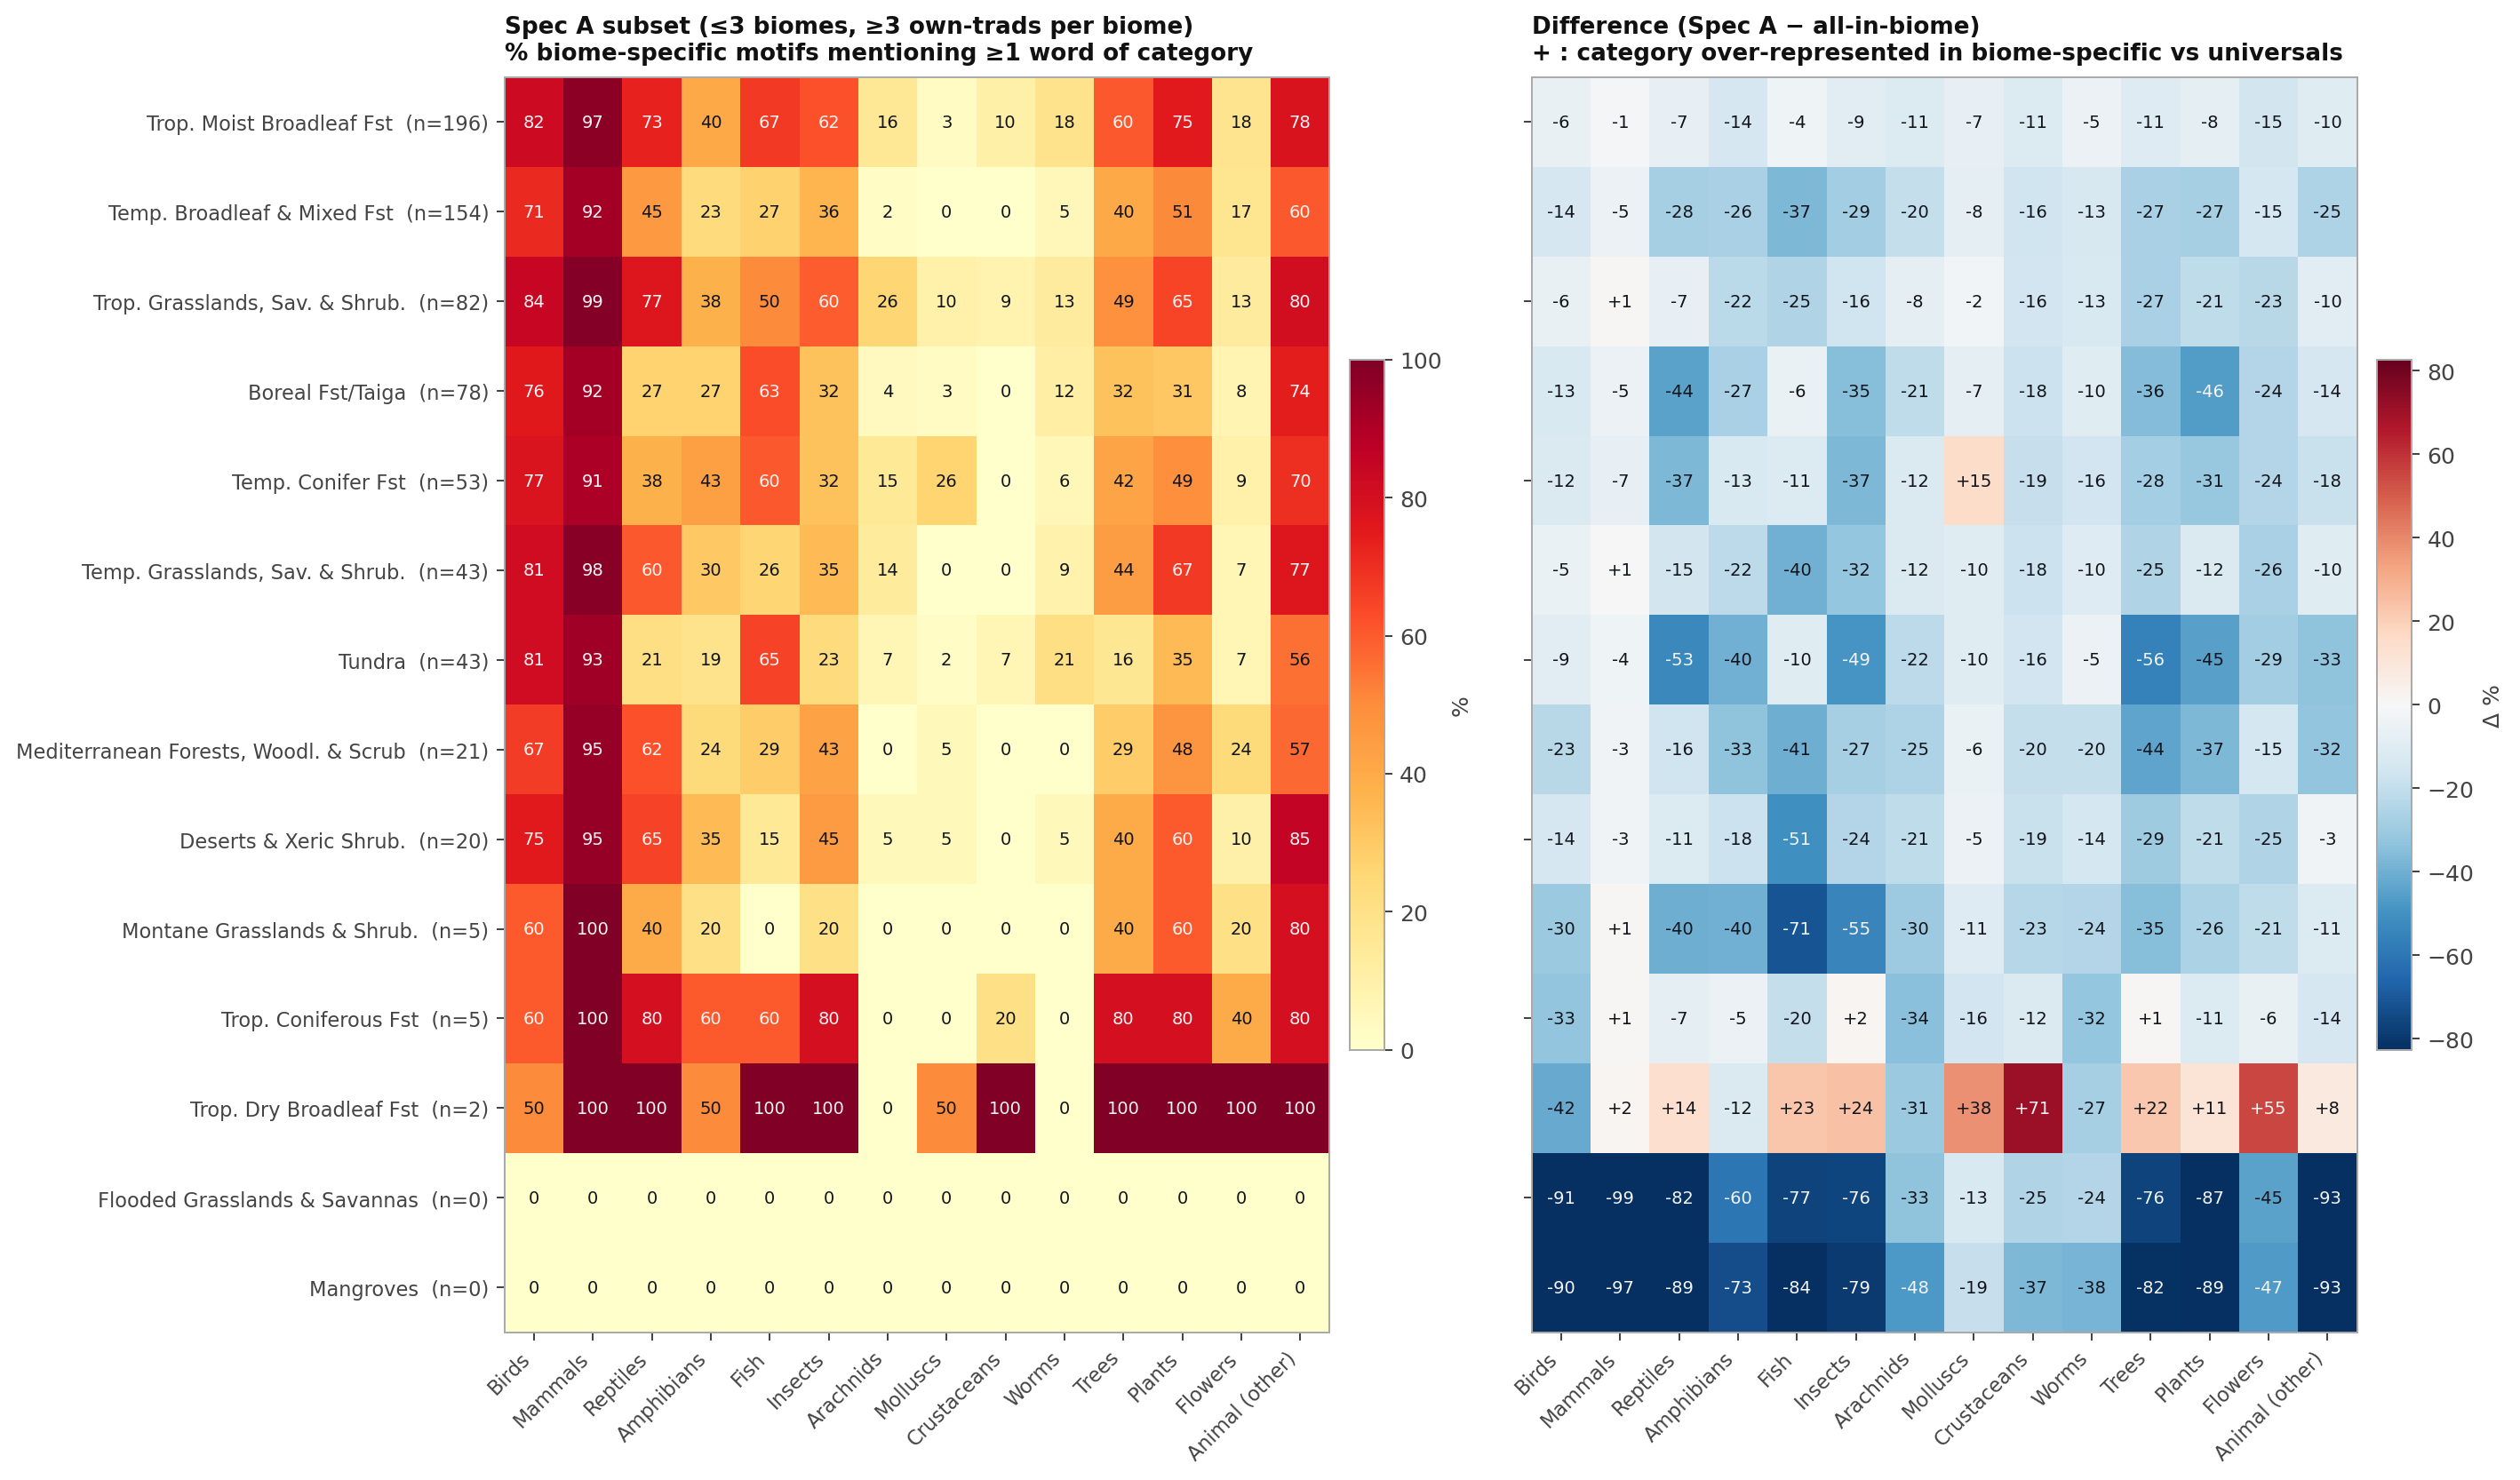
\includegraphics[width=0.95\textwidth]{figS_species_per_biome_specA.png}
\caption{\textbf{Ecological composition per biome (Spec~A subset).}
\emph{Left}: for each WWF biome (rows) and each of 14 taxonomic and
botanical categories (columns), the cell shows the percentage of
\emph{Spec~A motifs} (motifs touching $\leq 3$ biomes, $\geq 3$
own-traditions in that biome, the same selection that drives the
headline result) whose raw Russian abstract mentions at least one
species or plant of that category, before anonymisation.
\emph{Right}: difference (Spec~A minus all-in-biome). Positive cells
mark categories over-represented in biome-specific motifs relative
to the universal-dominated full pool, revealing the ecological
fingerprint that the species-hypernymisation layer subsequently
removes. The all-motifs version of the heatmap is dominated by
universal motifs and therefore uniformly red across biomes; we omit
it here and release the underlying counts in the data drop.}
\label{fig:figS-species}
\end{figure}

\end{document}
